\documentclass[11pt,a4paper]{article}

\usepackage[margin=2.2cm]{geometry}
\usepackage[T1]{fontenc}
\usepackage[utf8]{inputenc}
\usepackage{lmodern}
\usepackage{amsmath,amssymb,amsfonts}
\usepackage{graphicx}
\usepackage{booktabs}
\usepackage{array}
\usepackage{caption}
\usepackage{subcaption}
\usepackage{float}
\usepackage{hyperref}
\usepackage{xcolor}
\usepackage{microtype}
\usepackage{verbatim}

\hypersetup{
    colorlinks=true,
    linkcolor=black,
    citecolor=green!45!black,
    urlcolor=blue!60!black
}

\title{\textbf{High-Fidelity Multiphase Lattice Boltzmann Simulation and V\&V Analysis of a T-Junction Micro-Injector}}
\author{Computational Fluid Dynamics Portfolio Report \\ \small Solver: TCLB (\texttt{d2q9\_csf\_viscstep} / \texttt{d2q9\_csf\_viscstep\_cumulant})}
\date{\today}

\begin{document}

\maketitle

\begin{abstract}
This report presents a verified numerical investigation of two-phase droplet generation in a 2D T-junction micro-injector using the GPU-accelerated Lattice Boltzmann solver TCLB. A conservative Allen-Cahn phase-field model coupled with a Continuum Surface Force (CSF) formulation and smooth hyperbolic-tangent viscosity interpolation is validated against three canonical component benchmarks following a structured Verification and Validation (V\&V) methodology: the Young-Laplace static droplet law ($\sigma_{\mathrm{num}} = 0.08857$, $-1.59\%$ error, $R^2 = 0.9988$), sessile droplet wetting equilibrium ($59.08^\circ$, $89.26^\circ$, and $139.67^\circ$ for targets of $60^\circ$, $90^\circ$, and $143.24^\circ$), and 2D Poiseuille channel flow (profile shape $L_2$ error $0.061\%$, effective viscosity error $+0.70\%$). A five-point parametric sweep over the continuous-phase capillary number ($Ca \in [0.0050, 0.0117]$, $We \in [0.137, 0.745]$) captures the transition from confined slugging ($L_{\mathrm{slug}}/H > 1$) to steady shear-dominated dripping, yielding a tight power-law scaling for the dimensionless Sauter mean diameter, $D_{21}/H = 0.0149\,Ca^{-0.850}$ ($R^2 = 0.9997$), and breakup length, $L_b/H = 0.0246\,Ca^{-1.140}$ ($R^2 = 0.9807$). A grid independence study at refinement ratio $r = 1.5$ ($1280 \times 64$ vs. $1920 \times 96$) demonstrates topological invariance and a $48.2\%$ reduction in in-flight mass drift (effective order $p = 1.62$). Finally, replacing the Multi-Relaxation-Time (MRT) collision operator with the Cumulant operator reduces in-flight diameter drift by $10.7\times$ ($-1.60\%/100\text{ LU}$ to $+0.15\%/100\text{ LU}$), cuts droplet-to-droplet scatter by $65.5\%$, and suppresses low-viscosity acoustic pressure oscillations by two orders of magnitude.
\end{abstract}

\tableofcontents
\clearpage

% ==============================================================================
\section{Introduction and Engineering Objectives}
% ==============================================================================

Controlled atomization and monodisperse droplet generation in cross-flowing geometries are central to aerospace propulsion micro-injectors, liquid-fuel emulsification, and microfluidic reactors. In a T-junction injector, a dispersed fuel phase enters perpendicularly through a side branch of width $D$ into a continuous cross-flow channel of height $H$. The interplay between viscous shear, interfacial tension, confinement-induced pressure buildup, and wall wettability determines whether the injector operates in the \emph{squeezing}, \emph{dripping}, or \emph{jetting} regime.

The objective of this study is to establish a fully automated, reproducible, and rigorously verified Computational Fluid Dynamics (CFD) workflow using the open-source Lattice Boltzmann framework TCLB. Rather than relying on unverified qualitative visualizations, the methodology follows a four-stage Verification and Validation (V\&V) structure:
\begin{enumerate}
    \item \textbf{Component Verification:} Independent calibration of interfacial tension, contact angle hysteresis, effective viscosity, and boundary condition accuracy through Young-Laplace, sessile drop, and Poiseuille benchmarks.
    \item \textbf{Parametric Scaling Study:} Automated dual-probe optical tracking across five cross-flow velocities to extract dimensionless scaling laws for Sauter mean diameter ($D_{21}/H$), jet breakup length ($L_b/H$), and Strouhal number ($St$).
    \item \textbf{Grid Independence Study (GIS):} Constant-surface-tension mesh refinement ($r = 1.5$) with Richardson extrapolation and Grid Convergence Index (GCI) uncertainty quantification.
    \item \textbf{Collision Operator Assessment:} Direct quantitative comparison between the standard Multi-Relaxation-Time (MRT) and Cumulant collision operators under identical physical and geometric parameters.
\end{enumerate}

Detailed mathematical derivations, discretization choices, and physical justifications for all theoretical models used in this work are compiled in Appendices~\ref{app:lbm}--\ref{app:vv}.

% ==============================================================================
\section{Numerical Setup and Automated Measurement Methodology}
% ==============================================================================

\subsection{Computational Domain and Physical Parameters}

The injector geometry consists of a horizontal main channel of length $L_x = 1280\text{ LU}$ and interior height $H = 38\text{ LU}$ ($y \in [25, 62]$), intersected from below by a vertical fuel nozzle of width $D = 32\text{ LU}$ ($x \in [60, 91]$, aspect ratio $D/H = 0.842$) and depth $25\text{ LU}$. The overall lattice dimensions ($1280 \times 64$ for the baseline grid $G_1$ and $1920 \times 96$ for the refined grid $G_2$) are exact multiples of the CUDA block size ($32 \times 16$), eliminating warp padding overhead on the NVIDIA GTX~745 GPU.

\begin{table}[H]
\caption{Baseline physical and numerical parameters in lattice units (LU) for grid $G_1$ ($1280 \times 64$).}
\label{tab:setup}
\hspace{-1.5cm}
\begin{tabular}{@{}llll@{}}
\toprule
\textbf{Parameter} & \textbf{Symbol / TCLB Name} & \textbf{Value} & \textbf{Physical Meaning} \\
\midrule
Channel height / Nozzle width & $H$ / $D$ & $38$ / $32\text{ LU}$ & Confinement ratio $D/H = 0.842$ \\
Continuous-phase viscosity & $\nu_c$ (\texttt{Viscosity}) & $0.025$ & Relaxation rate $\omega_c = 1.739$ \\
Dispersed-phase viscosity & $\nu_d$ (\texttt{Viscosity\_l}) & $0.012$ & Viscosity ratio $\lambda = \nu_d/\nu_c = 0.48$ \\
Viscosity transition width & \texttt{ViscosityStepWidth} & $0.25$ & Smooth $\tanh$ interpolation across $\phi$ \\
Nominal surface tension & $\sigma$ (\texttt{SurfaceTensionRate}) & $0.090$ & Capillary wave speed $c_{\mathrm{cap}} = 0.376 < c_s$ \\
Phase-field mobility & $M$ (\texttt{Mobility}) & $0.010$ & Relaxation rate $\omega_\phi = 1.887$ \\
Inverse interface width & $W$ (\texttt{IntWidth}) & $0.333$ & 10\%--90\% thickness $\approx 3.30\text{ LU}$ \\
Nominal contact angle & $\theta$ (\texttt{WettingAngle}) & $2.50\text{ rad}$ & Non-wetting wall ($\theta = 143.24^\circ$) \\
Wall adhesion factor & \texttt{WallAdhesionDecay} & $0.70$ & Active near-wall capillary repulsion \\
Dispersed inlet velocity & $U_d$ (\texttt{VelocityY}) & $0.008$ & Constant fuel flux $Q_d = 0.256\text{ LU}^2/\text{it}$ \\
Continuous inlet velocity & $U_c$ (\texttt{VelocityX}) & $0.018\text{--}0.042$ & Parametric sweep variable \\
\bottomrule
\end{tabular}
\end{table}

No-slip walls are enforced via halfway bounce-back (\texttt{Wall}), continuous and dispersed inlets use Zou-He velocity boundaries (\texttt{WVelocity}, \texttt{SVelocity}), and the right boundary imposes a constant-pressure outflow (\texttt{EPressure}, $P = 0$). Because the standard \texttt{EPressure} boundary in \texttt{d2q9\_csf} fixes a Dirichlet phase value ($\phi = -0.5$), the total simulation duration for each case is scaled inversely with the downstream mixture velocity $U_{\mathrm{down}} = U_c + U_d(D/H)$ so that at least three droplets form while the leading droplet terminates with a $\sim 180\text{ LU}$ safety buffer upstream of the outlet.

\subsection{Automated Dual-Probe Optical Tracking}

To eliminate subjective visual sizing and path-length bias caused by phase-field diffusion, a dedicated Python post-processing pipeline (\texttt{analyze\_droplets.py}) evaluates each VTI snapshot as follows:
\begin{enumerate}
    \item \textbf{Wall Masking and Iso-Contour Extraction:} Solid wall nodes (where \texttt{getPhaseField()} returns $0.0$) are masked to $-0.5$ before thresholding strictly at the physical zero contour $\phi > 0.0$, reducing discretization sizing bias to $< 0.05\text{ LU}$.
    \item \textbf{Breakup Detection:} The body connected to the nozzle ($y_{\min} < 10\text{ LU}$) yields the instantaneous attached jet length $L_b(t) = x_{\max} - x_{\mathrm{nozzle}}$. Sudden retractions $\Delta L_b > 30\text{ LU}$ identify pinch-off events.
    \item \textbf{Relative Dual-Probe Tracking:} Two virtual optical probes are placed automatically downstream of the steady breakup point at $P_1 = x_{\mathrm{nozzle}} + \overline{L}_b + 110\text{ LU}$ and $P_2 = P_1 + 200\text{ LU}$. Individual droplets (area $\ge 50$ cells to reject satellite artifacts) are tracked across frames and linearly interpolated at exact probe crossings to measure equivalent diameter $D_{\mathrm{eq}} = 2\sqrt{A/\pi}$, aspect ratio $AR = \Delta x / \Delta y$, droplet velocity $U_{\mathrm{drop}}$, shedding period $T_{P1}$, and normalized diameter drift per $100\text{ LU}$ of flight. The first startup droplet is explicitly tagged and excluded from steady-state statistics.
\end{enumerate}

% ==============================================================================
\section{Component Verification Benchmarks}
% ==============================================================================

Before evaluating injector dynamics, the compiled solver (\texttt{d2q9\_csf\_viscstep}) was subjected to three independent analytical benchmarks. The combined MRT verification results are presented in Figure~\ref{fig:bm_mrt} and summarized in Table~\ref{tab:benchmarks}.

\begin{figure}[H]
    \centering
    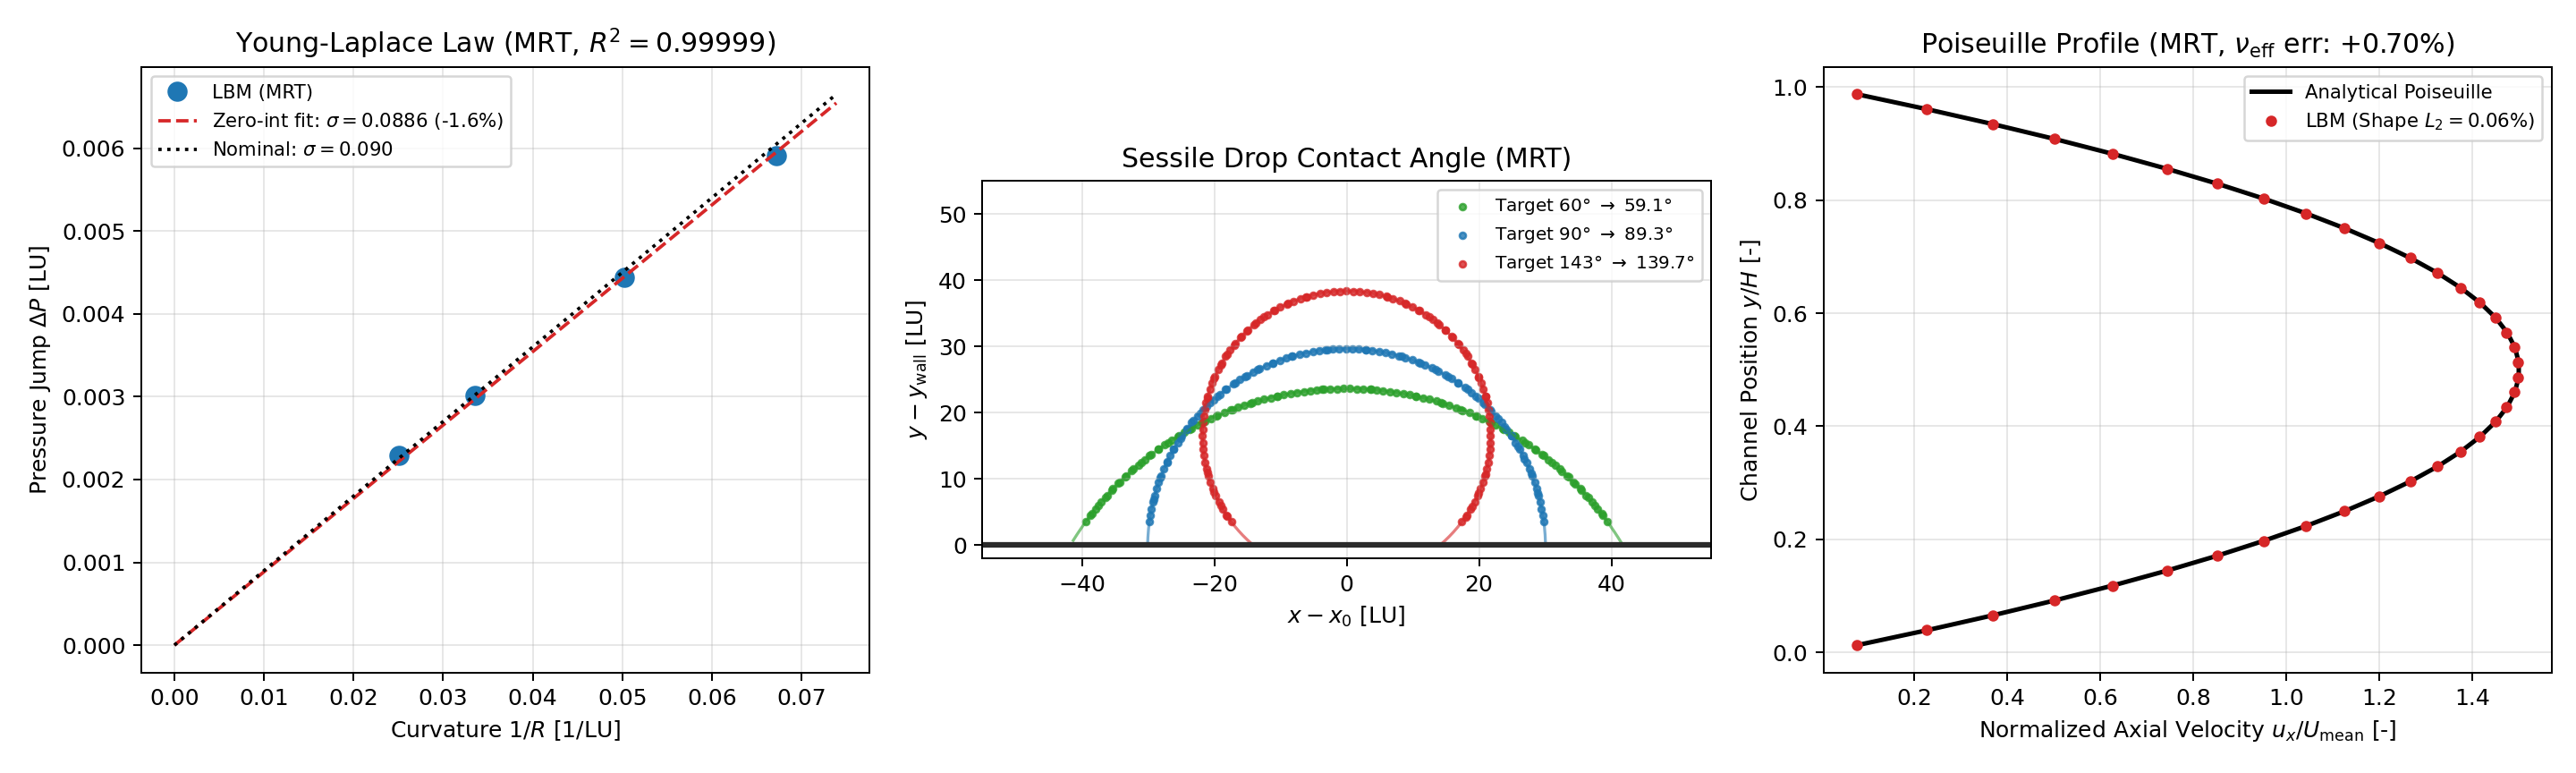
\includegraphics[width=\textwidth]{benchmarks/validation_benchmarks.png}
    \caption{Component verification benchmarks for the baseline MRT solver (\texttt{d2q9\_csf\_viscstep}): (left) Young-Laplace capillary pressure jump vs. curvature $1/R$, (center) sessile droplet equilibrium profiles and circular fits for $\theta = 60^\circ, 90^\circ, 143.2^\circ$, and (right) developed 2D Poiseuille velocity profile at $x = 250\text{ LU}$.}
    \label{fig:bm_mrt}
\end{figure}

\subsection{Young-Laplace Law and Spurious Currents}

Static circular droplets of initial radii $R \in \{15, 20, 30, 40\}\text{ LU}$ were initialized in a $160 \times 160$ periodic domain with a 500-step zero-tension interface smoothing phase followed by $15\,000$ capillary relaxation steps at $\sigma_{\mathrm{nom}} = 0.090$. To properly damp radial acoustic waves generated by the step activation of surface tension in a closed periodic box, the static test was performed at $\nu = 1/6$ ($\omega = 1.0$, acoustic damping time $\tau_{\mathrm{ac}} \approx 3890\text{ it}$), yielding core density standard deviations below $2.8 \times 10^{-5}$.

The measured pressure jump $\Delta P = (\bar{\rho}_{\mathrm{in}} - \bar{\rho}_{\mathrm{out}})/3$ exhibits excellent linearity against $1/R_{\mathrm{eq}}$ ($R^2 = 0.999992$ for free-intercept regression, $b = +0.000137$). The physically constrained zero-intercept regression ($\Delta P = \sigma_{\mathrm{num}}/R$) gives $\sigma_{\mathrm{num}} = 0.08857$ (error $-1.59\%$ relative to $\sigma_{\mathrm{nom}} = 0.090$), while pointwise values $\sigma_i = \Delta P \cdot R_{\mathrm{eq}}$ range from $0.08793$ ($R=15$) to $0.09141$ ($R=40$) with a mean of $0.08942$ ($-0.64\%$). Maximum spurious velocities remain bounded at $\max|\mathbf{U}_{\mathrm{sp}}| \le 4.77 \times 10^{-3}\text{ LU}$.

\subsection{Sessile Drop Wetting Equilibrium}

Equilibrium contact angles were measured on a $192 \times 96$ walled channel using identical wall parameters to the injector (\texttt{WallAdhesionDecay = 0.7}) for target angles of $60^\circ$, $90^\circ$, and $143.24^\circ$ ($2.50\text{ rad}$). Sub-pixel extraction of the $\phi = 0.0$ contour above the near-wall layer ($y \ge 4$) and algebraic circle fitting yield circularity RMS residuals of only $0.007\text{--}0.013\text{ LU}$. Measured angles match target values within $1^\circ$ for hydrophilic and neutral walls ($59.08^\circ$ and $89.26^\circ$) and reach $139.67^\circ$ (error $-3.57^\circ$) in the strongly hydrophobic regime used in the T-junction.

\subsection{2D Poiseuille Channel Flow}

A single-phase channel ($320 \times 40$, $H = 38\text{ LU}$, $\nu_c = 0.025$, $U_c = 0.028$, $Re = 42.56$) was pre-initialized with uniform axial velocity $U_c$ to eliminate quarter-wave startup acoustic transients and simulated for $25\,000$ iterations. Sampled at $x = 250\text{ LU}$ (well beyond the hydrodynamic entrance length $L_e \approx 0.05\,Re\,H \approx 81\text{ LU}$), the normalized profile matches the analytical parabola with a shape error of $L_2 = 0.061\%$ and total $L_2 = 0.740\%$ (the $+0.78\%$ local mean velocity increase is primarily physical weak-compressibility acceleration due to the axial density drop $\rho_1/\rho_{250} = 1.0056$). Mass flux is conserved within $+0.068\%$ from inlet to outlet, and the effective kinematic viscosity extracted from the developed pressure gradient ($x \in [250, 318]$) is $\nu_{\mathrm{eff}} = 0.02518$ (error $+0.70\%$).

\begin{table}[H]
\caption{Summary of component verification benchmarks and calibration uncertainties (MRT solver).}
\label{tab:benchmarks}
\hspace{-1.5cm}
\begin{tabular}{@{}llll@{}}
\toprule
\textbf{Benchmark} & \textbf{Reference / Target} & \textbf{Measured (MRT)} & \textbf{Relative / Abs. Error} \\
\midrule
Young-Laplace $\sigma_{\mathrm{num}}$ (zero-int) & $\sigma_{\mathrm{nom}} = 0.09000$ & $0.08857$ ($R^2 = 0.9988$) & $-1.59\%$ \\
Young-Laplace $\sigma_{\mathrm{fit}}$ (free-int) & $\sigma_{\mathrm{nom}} = 0.09000$ & $0.08583$ ($b = +1.37\times 10^{-4}$) & $-4.64\%$ \\
Sessile drop ($\theta = 60.00^\circ$) & $60.00^\circ$ & $59.08^\circ$ ($\text{RMS} = 0.007\text{ LU}$) & $-0.92^\circ$ \\
Sessile drop ($\theta = 90.00^\circ$) & $90.00^\circ$ & $89.26^\circ$ ($\text{RMS} = 0.012\text{ LU}$) & $-0.74^\circ$ \\
Sessile drop ($\theta = 143.24^\circ$, injector) & $143.24^\circ$ & $139.67^\circ$ ($\text{RMS} = 0.013\text{ LU}$) & $-3.57^\circ$ ($-2.49\%$) \\
Poiseuille velocity shape $L_2$ & $0.000\%$ & $0.061\%$ (total $L_2 = 0.740\%$) & $< 0.1\%$ shape error \\
Poiseuille effective viscosity $\nu_{\mathrm{eff}}$ & $\nu_c = 0.02500$ & $0.02518$ & $+0.70\%$ \\
\midrule
\multicolumn{4}{@{}l@{}}{\small \textit{Propagated dimensionless calibration uncertainty:} $\Delta Ca / Ca \approx +2.36\%$, $\Delta We / We \approx +1.63\%$.} \\
\bottomrule
\end{tabular}
\end{table}

% ==============================================================================
\section{T-Junction Micro-Injector Dynamics and Parametric Sweep}
% ==============================================================================

\subsection{Baseline Flow Physics ($U_c = 0.028$, $Ca = 0.0078$)}

Figure~\ref{fig:flow_fields} illustrates the coupled multi-field structure of the baseline case at $t = 36\,000$. The hydrophobic wall condition ($\theta_{\mathrm{num}} \approx 139.7^\circ$) maintains a thin lubricating film of continuous phase beneath the emerging fuel jet and around detached droplets. As the fuel tip expands upward into the main channel, streamlines compress above the crest, locally accelerating the continuous phase to $|\mathbf{U}|/U_c \approx 1.8\text{--}2.0$. This local constriction builds upstream pressure and viscous shear, thinning the neck until capillary retraction pinches off a spherical droplet ($AR = 1.01$, $D_{21}/H = 0.922$).

\begin{figure}[H]
    \centering
    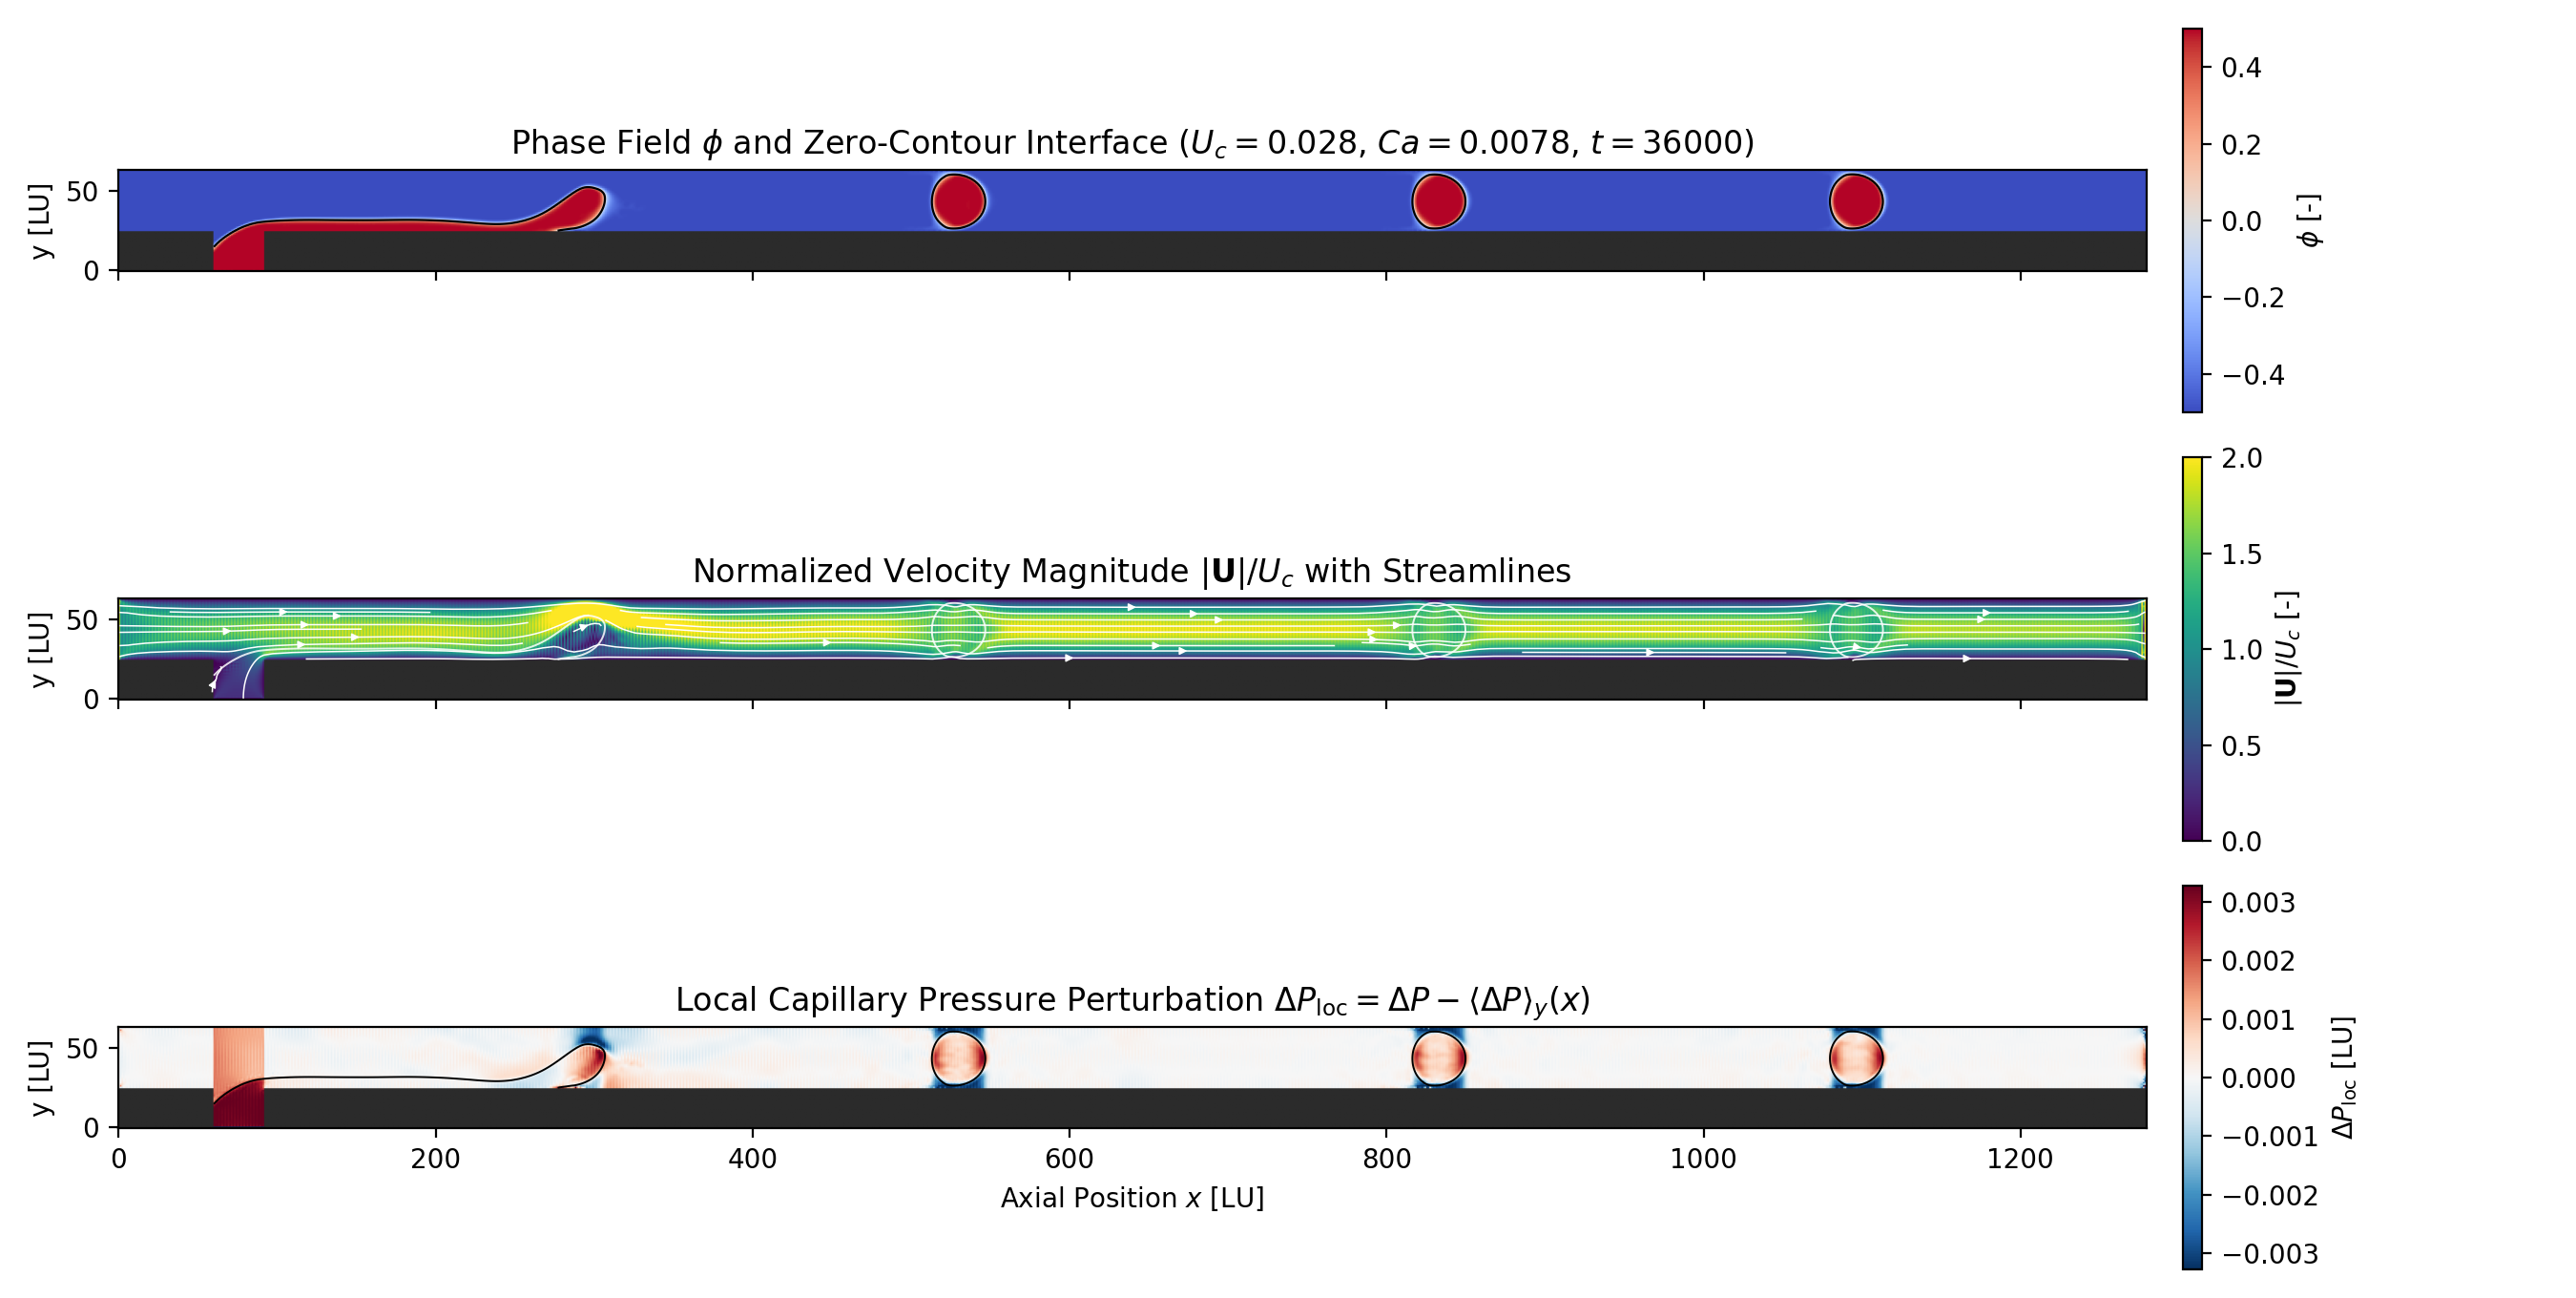
\includegraphics[width=1.1\textwidth]{sweep/Uc_0.028/flow_fields_baseline.png}
    \caption{Multi-field visualization of the baseline micro-injector ($U_c = 0.028$, $Ca = 0.0078$, $t = 36\,000$): phase field $\phi$, normalized velocity magnitude $|\mathbf{U}|/U_c$ with streamlines, and local capillary pressure perturbation showing the Laplace pressure jump inside detached droplets.}
    \label{fig:flow_fields}
\end{figure}

Figure~\ref{fig:telemetry} shows the sawtooth time series of the attached jet length $L_b(t)$ for the baseline case. Following the initial startup pinch-off at $t = 11\,500$ ($L_b = 185\text{ LU}$), the cycle settles into repeatable periodic shedding at $t = 22\,000$ and $t = 31\,000$, with probe crossing intervals of $8134\text{ it}$ ($St = 0.1668$) and droplet-to-droplet diameter standard deviation of $2.55\%$.

\begin{figure}[H]
    \centering
    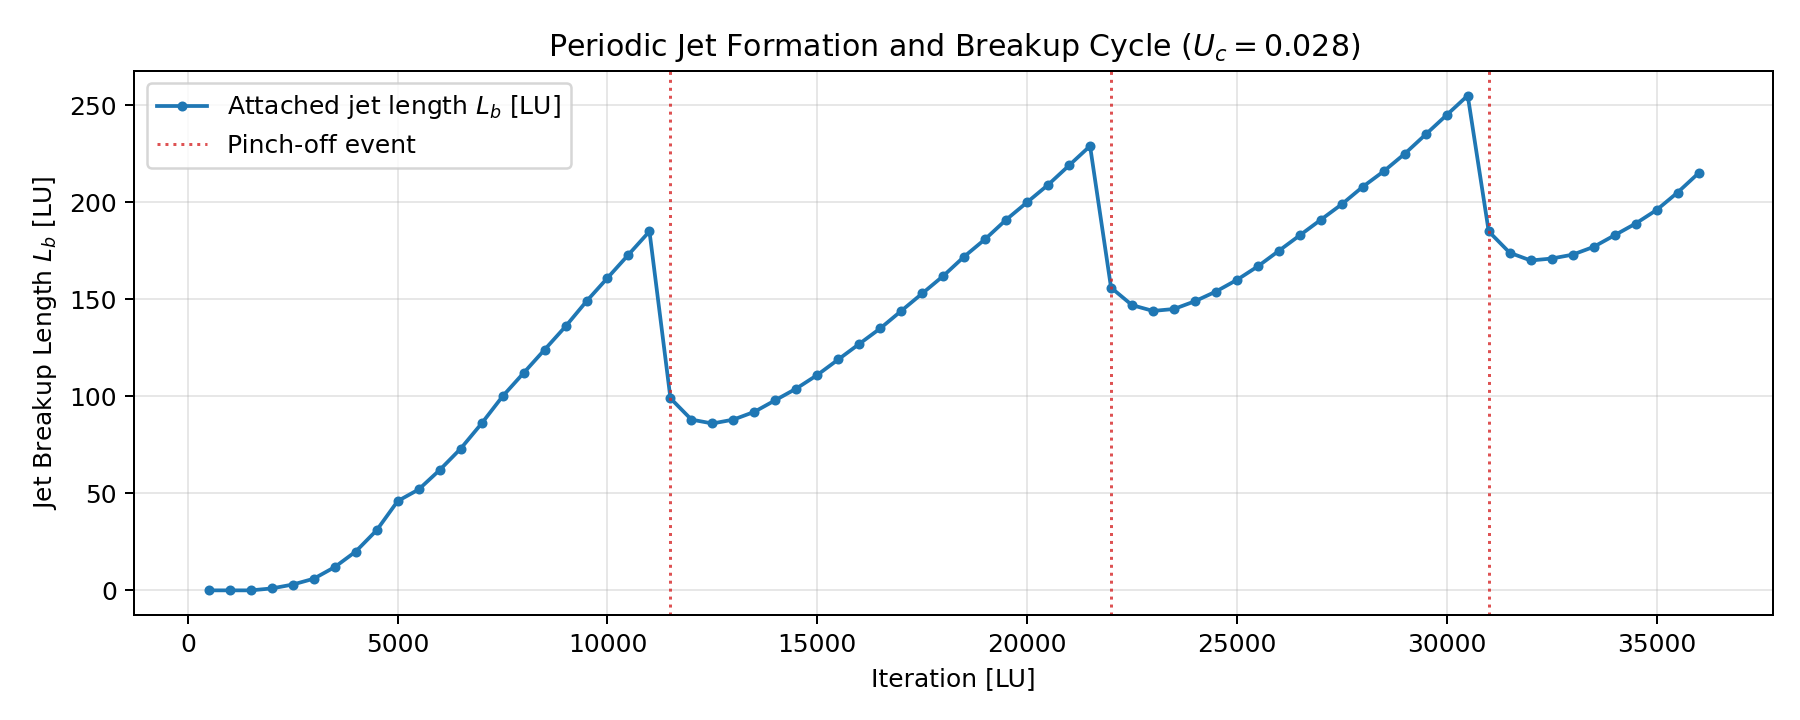
\includegraphics[width=0.92\textwidth]{sweep/Uc_0.028/breakup_telemetry.png}
    \caption{Time evolution of attached jet length $L_b(t)$ for the baseline case ($U_c = 0.028$), illustrating periodic jet growth and sudden retraction at pinch-off events (vertical dashed lines).}
    \label{fig:telemetry}
\end{figure}

\subsection{Parametric Sweep and Scaling Laws}

Five continuous-phase velocities ($U_c \in [0.018, 0.042]$) were simulated at constant fuel injection velocity ($U_d = 0.008$), spanning $Ca \in [0.0050, 0.0117]$, $We \in [0.137, 0.745]$, $Re_c \in [27.4, 63.8]$, and flow rate ratio $Q_d/Q_c \in [0.16, 0.37]$. All runs completed without numerical instabilities (\texttt{NaN = 0}). The final phase-field topologies are compared in Figure~\ref{fig:montage}, and full quantitative metrics are listed in Table~\ref{tab:sweep}.

\begin{figure}[H]
    \centering
    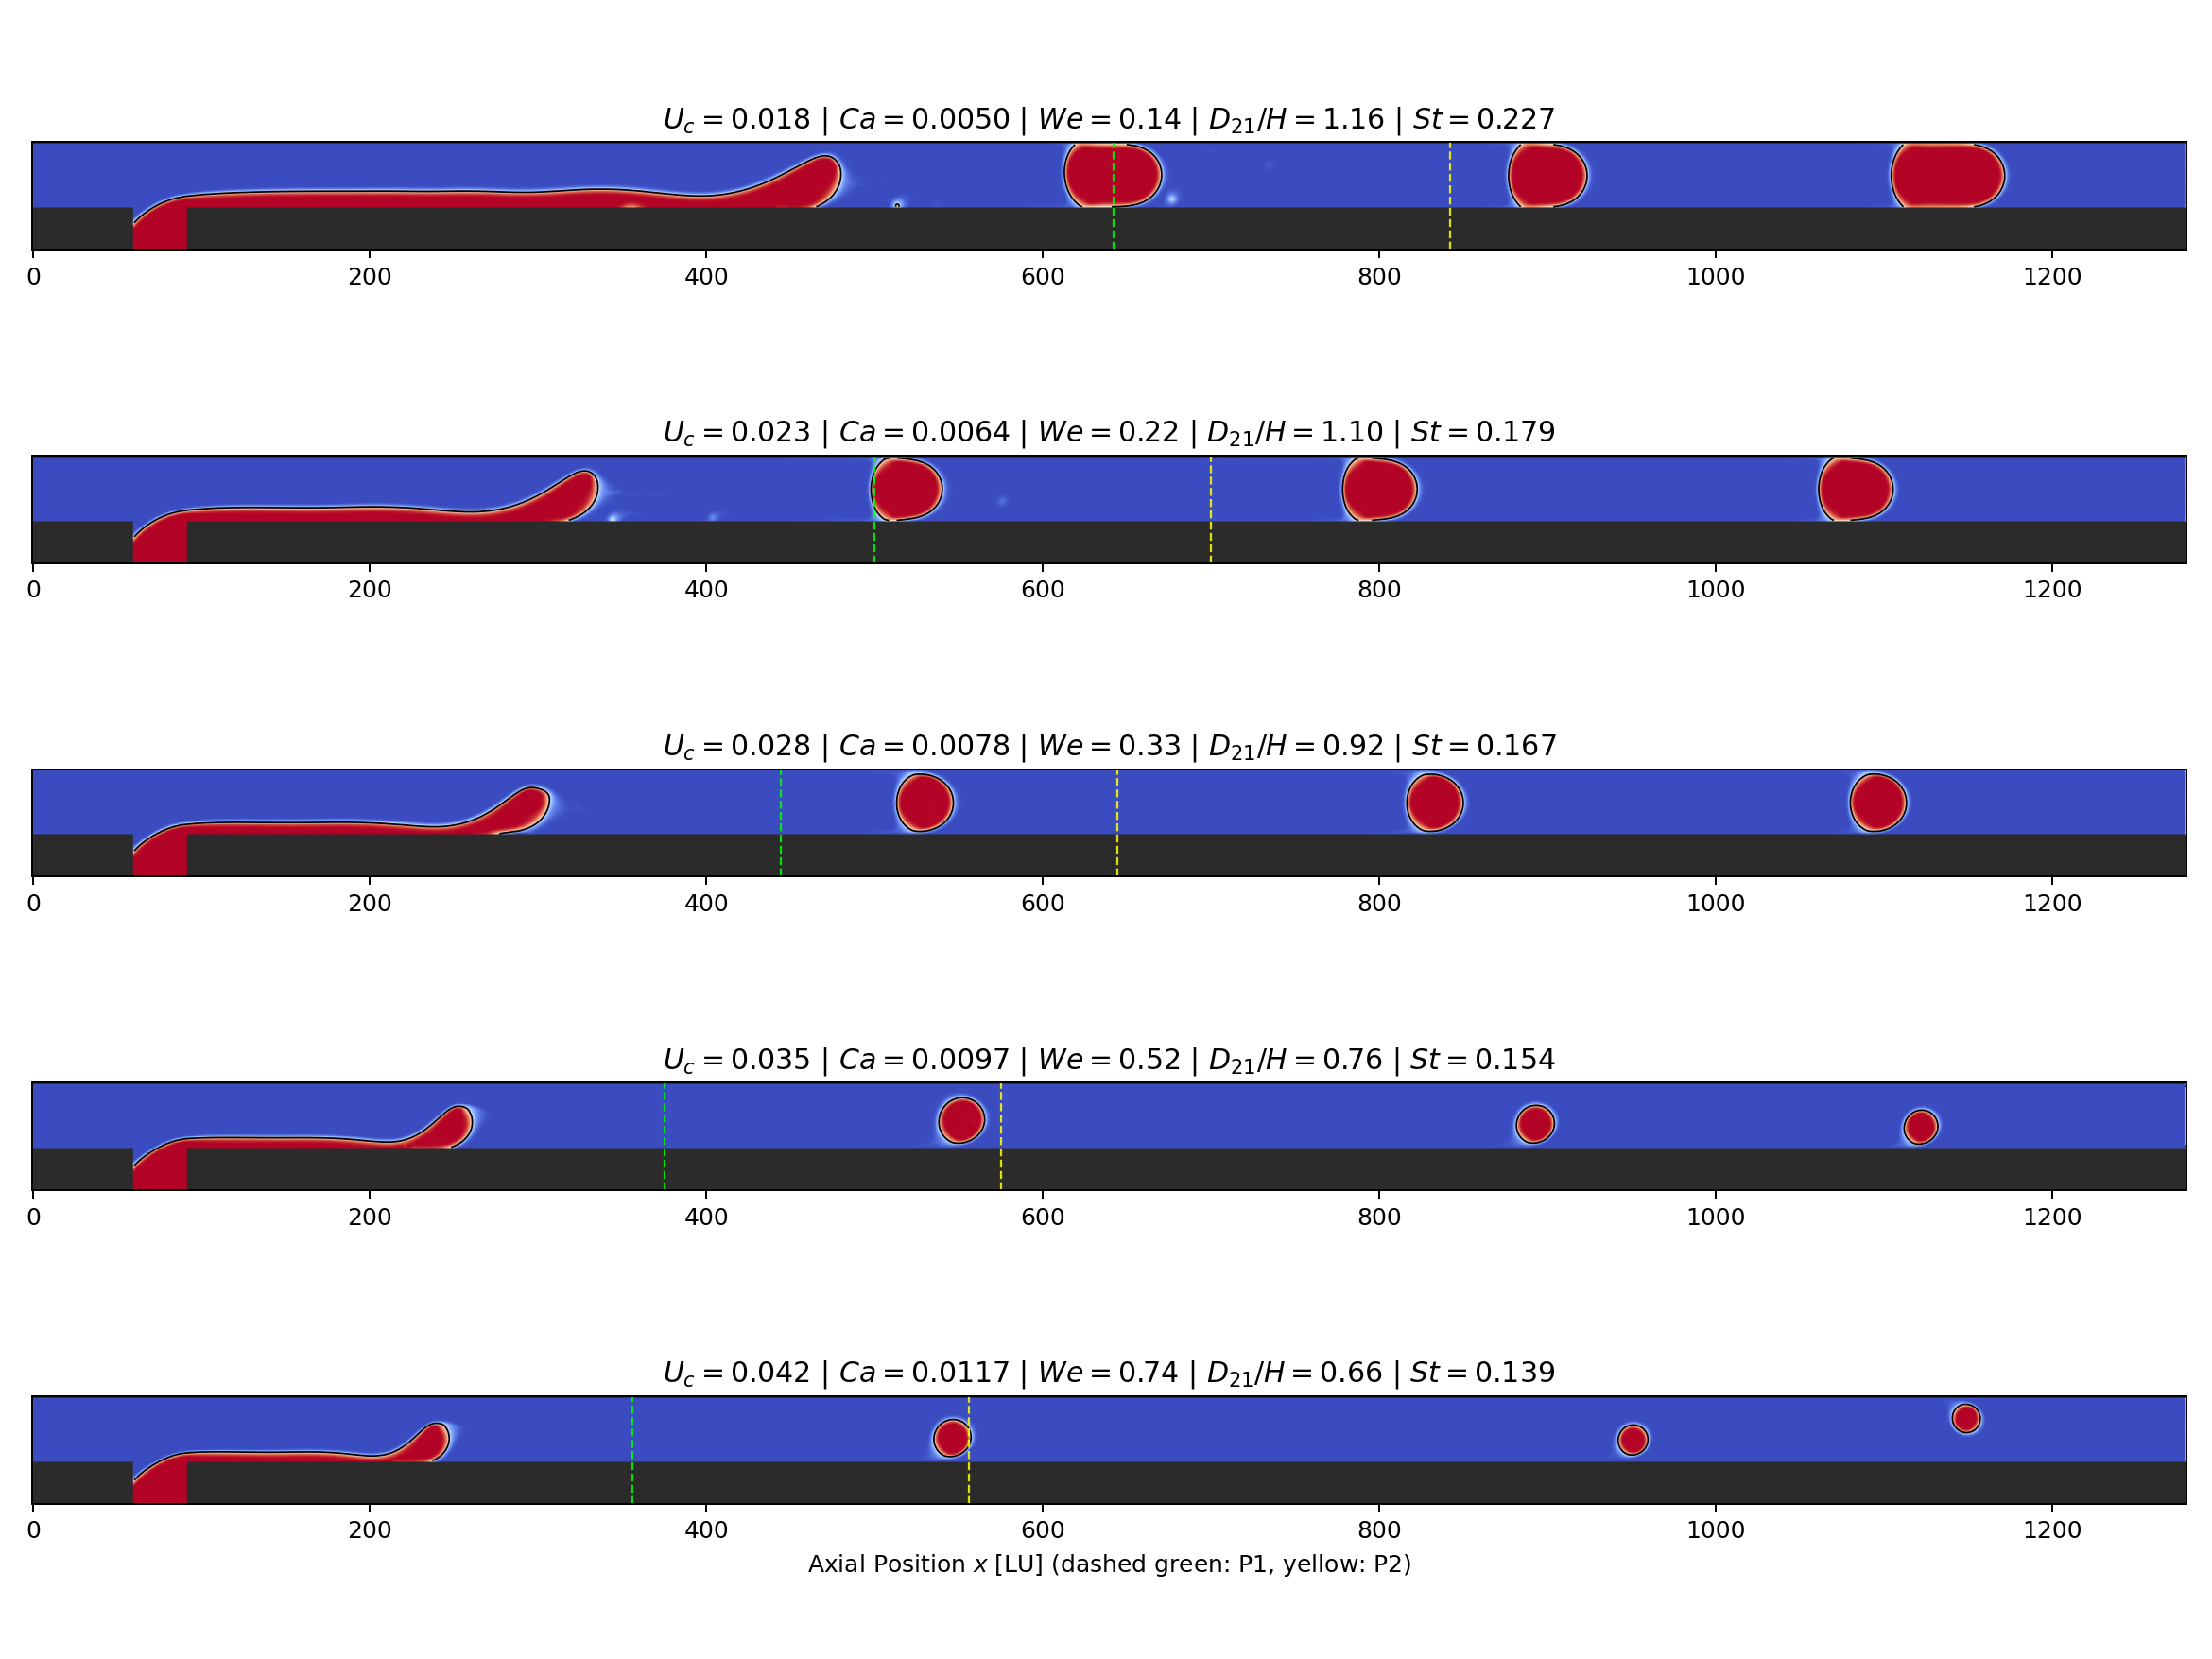
\includegraphics[width=\textwidth]{sweep/sweep_montage.png}
    \caption{Final phase-field snapshots across the five-point parametric sweep showing the morphological transition from elongated Taylor slugs ($U_c = 0.018$) to small spherical droplets ($U_c = 0.042$). Green and yellow dashed lines mark the adaptive optical probes $P_1$ and $P_2$.}
    \label{fig:montage}
\end{figure}

\begin{table}[H]
\caption{Aggregated parametric sweep results on grid $G_1$ ($1280 \times 64$, MRT operator, adaptive relative probes $P_1 = x_{\mathrm{nozzle}} + \overline{L}_b + 110\text{ LU}$).}
\label{tab:sweep}
\small
\hspace{-1.5cm}
\begin{tabular}{@{}cccccccccccc@{}}
\toprule
$U_c$ & $Ca$ & $We$ & $Re_c$ & $Q_d/Q_c$ & $D_{21}/H$ & $L_{\mathrm{slug}}/H$ & $L_b/H$ & $f$ [$10^{-4}\text{ it}^{-1}$] & $St$ & $AR$ & Drift [\%/100LU] \\
\midrule
$0.018^*$ & $0.0050$ & $0.137$ & $27.4$ & $0.374$ & $1.155$ & $1.263$ & $11.58$ & $1.07^*$ & $0.2267^*$ & $1.26$ & $-0.05$ \\
$0.023$   & $0.0064$ & $0.223$ & $35.0$ & $0.293$ & $1.098$ & $1.166$ & $7.83$  & $1.08$   & $0.1790$   & $1.17$ & $-0.89$ \\
$0.028$   & $0.0078$ & $0.331$ & $42.6$ & $0.241$ & $0.922$ & $0.921$ & $6.37$  & $1.23$   & $0.1668$   & $1.01$ & $-1.60$ \\
$0.035$   & $0.0097$ & $0.517$ & $53.2$ & $0.192$ & $0.764$ & $0.758$ & $4.55$  & $1.42$   & $0.1542$   & $0.99$ & $-5.16$ \\
$0.042$   & $0.0117$ & $0.745$ & $63.8$ & $0.160$ & $0.658$ & $0.658$ & $4.07$  & $1.54$   & $0.1390$   & $1.00$ & $-5.55$ \\
\bottomrule
\multicolumn{12}{@{}l@{}}{\footnotesize $^*$Transitional lower-boundary case: $L_b$ creeps downstream ($L_{b,2}=382\text{ LU} \to L_{b,3}=498\text{ LU}$); period includes startup drop \#1.}
\end{tabular}
\end{table}

As shown in Figures~\ref{fig:scaling} and~\ref{fig:regime}, increasing the continuous-phase cross-flow velocity produces monotonic reductions in both droplet size and breakup length, alongside a $43\%$ increase in dimensional shedding frequency ($f = 1.08 \to 1.54$ droplets per $10^4$ iterations). Because $U_c$ increases faster than $f$ at constant fuel supply $Q_d$, the dimensionless Strouhal number $St = fH/U_c$ decreases mildly from $0.1790$ to $0.1390$ across the steady regime.

\begin{figure}[H]
    \centering
    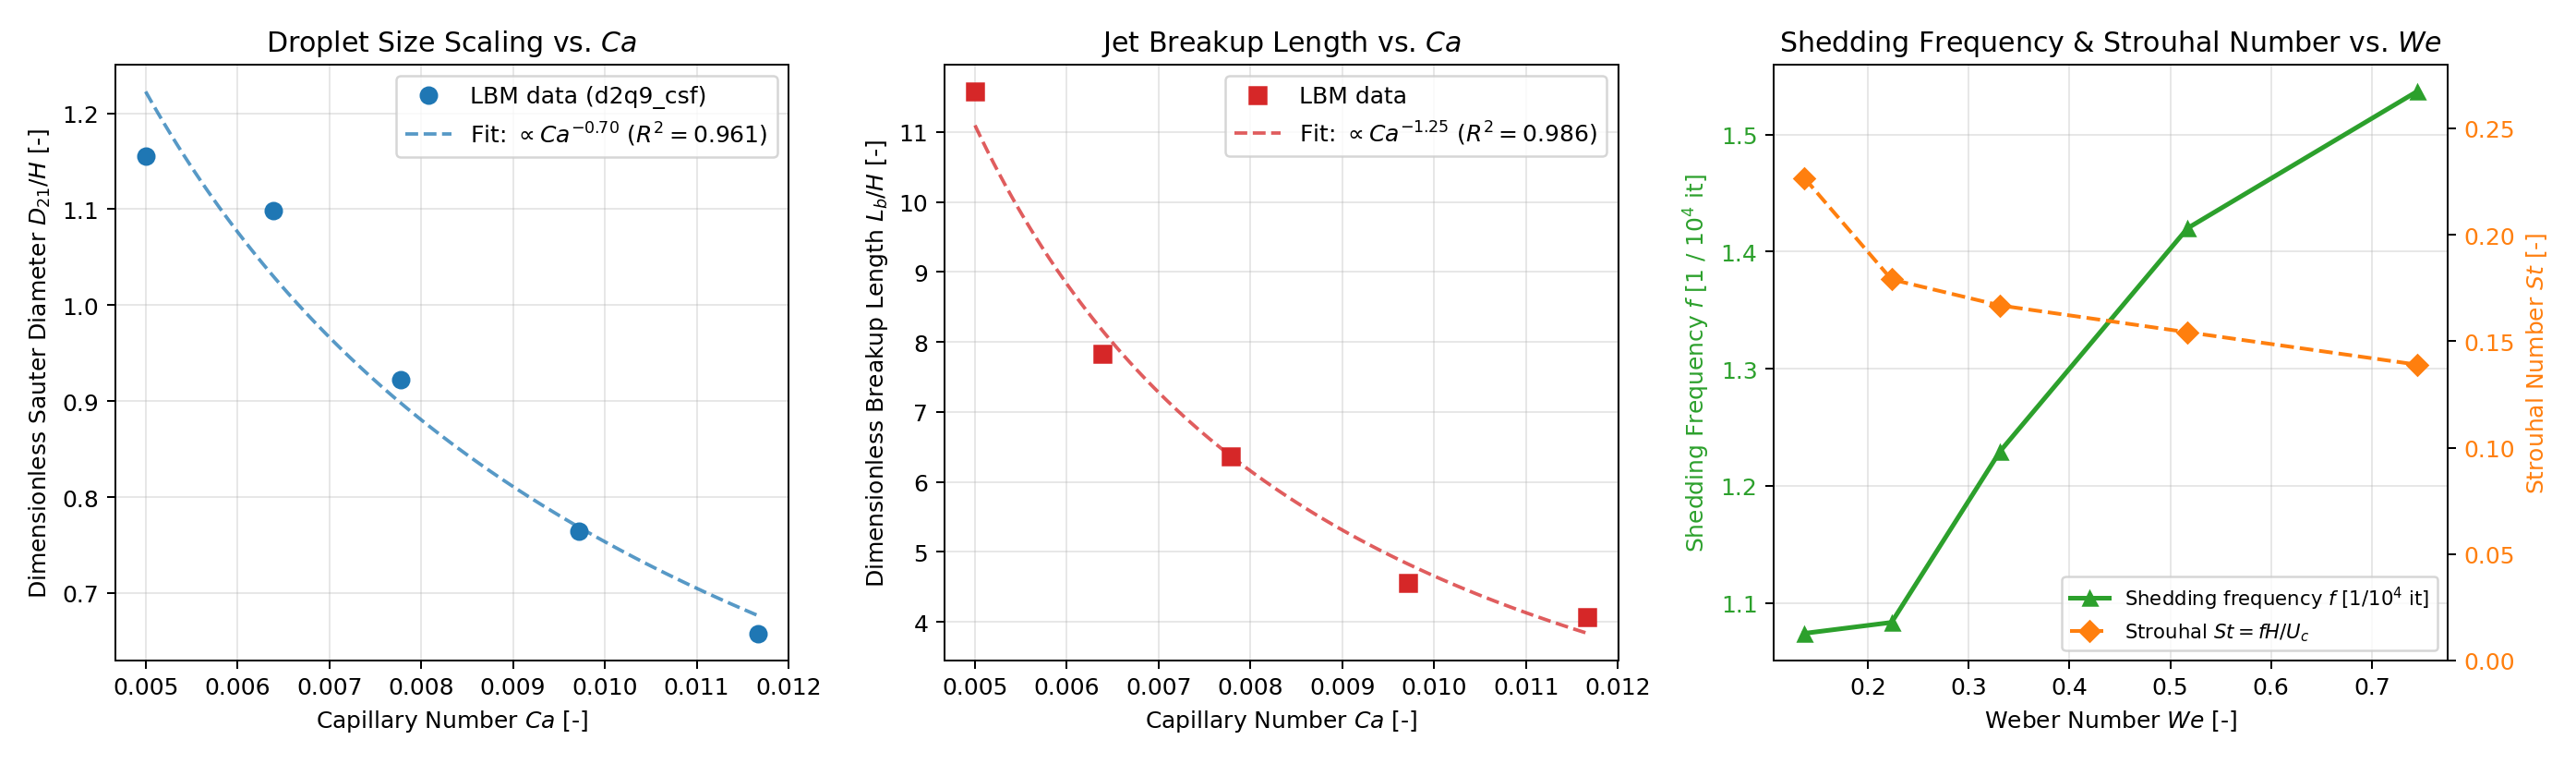
\includegraphics[width=\textwidth]{sweep/sweep_scaling.png}
    \caption{Dimensionless scaling trends across the parametric sweep: (left) Sauter mean diameter $D_{21}/H$ vs. $Ca$, (center) breakup length $L_b/H$ vs. $Ca$, and (right) dimensional shedding frequency $f$ and Strouhal number $St$ vs. $We$.}
    \label{fig:scaling}
\end{figure}

\begin{figure}[H]
    \centering
    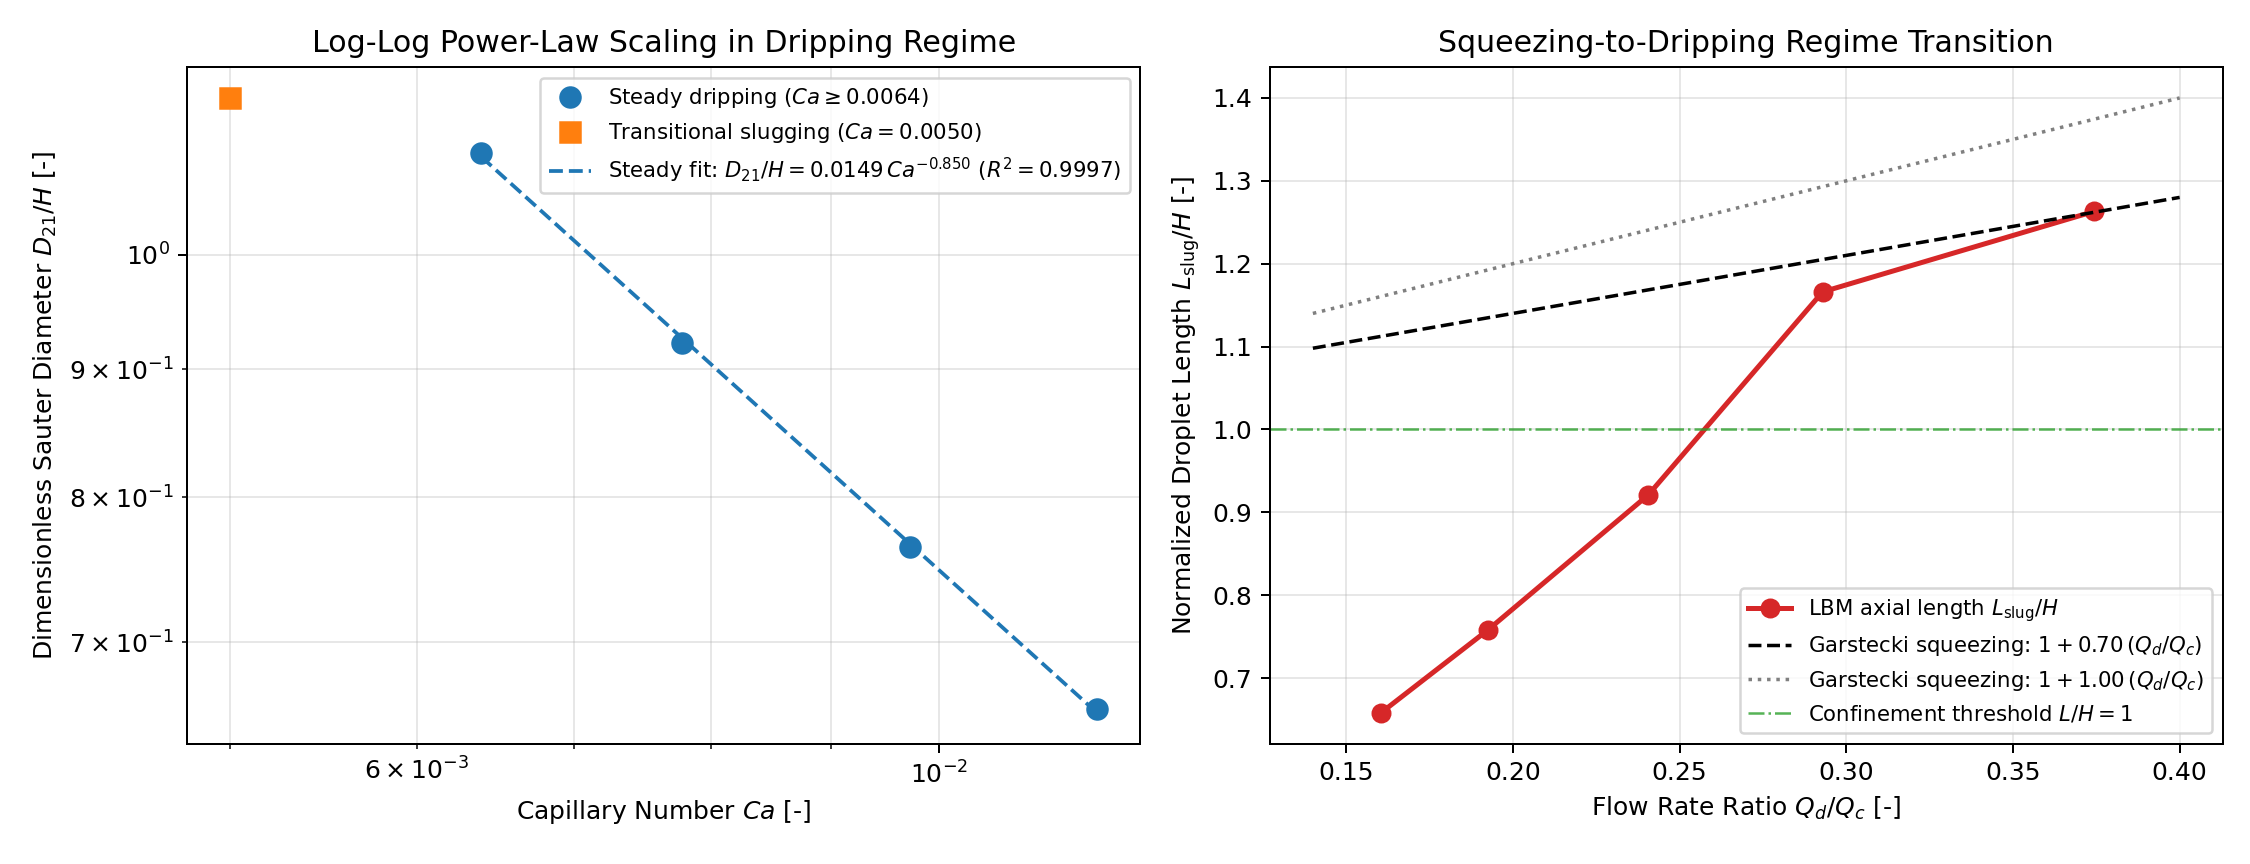
\includegraphics[width=\textwidth]{sweep/sweep_regime_analysis.png}
    \caption{Regime identification and literature comparison: (left) log-log power-law regression in the steady dripping regime ($R^2 = 0.9997$), and (right) axial droplet length $L_{\mathrm{slug}}/H$ vs. flow rate ratio $Q_d/Q_c$ compared against the Garstecki squeezing model $L/H = 1 + \alpha (Q_d/Q_c)$.}
    \label{fig:regime}
\end{figure}

Power-law regression across the four fully steady cases ($Ca \in [0.0064, 0.0117]$) yields:
\begin{align}
    \frac{D_{21}}{H} &= 0.0149\,Ca^{-0.850} = 0.5788\,We^{-0.425} && (R^2 = 0.9997), \\
    \frac{L_b}{H} &= 0.0246\,Ca^{-1.140} && (R^2 = 0.9807).
\end{align}
Including the lowest-$Ca$ transitional slugging point ($U_c = 0.018$, where channel confinement caps radial growth and shifts the droplet into an elongated slug with $AR = 1.26$) flattens the global exponent to $D_{21}/H = 0.0302\,Ca^{-0.698}$ ($R^2 = 0.9612$) and $L_b/H = 0.0145\,Ca^{-1.253}$ ($R^2 = 0.9856$). Figure~\ref{fig:regime} (right) clearly resolves the physical transition around $Q_d/Q_c \approx 0.25$ ($Ca \approx 0.007$): for $Q_d/Q_c \ge 0.29$, droplets fill the channel ($L_{\mathrm{slug}}/H > 1$) and approach the linear Garstecki squeezing law $L/H = 1 + 0.70(Q_d/Q_c)$; for $Q_d/Q_c \le 0.24$, droplets detach before full channel blockage ($L_{\mathrm{slug}}/H < 1$) and enter the shear-dominated dripping regime.

At the upper velocity end ($U_c = 0.035\text{--}0.042$), droplet diameter shrinks to $25\text{--}29\text{ LU}$ ($\sim 7.5$ interface widths), increasing curvature-driven phase-field drift to $-5.16\%\text{ to }-5.55\%/100\text{ LU}$ and scatter to $6.15\%$. This defines the practical resolution limit of the baseline $H = 38\text{ LU}$ grid under MRT.

% ==============================================================================
\section{Grid Independence Study (GIS)}
% ==============================================================================

Mesh convergence was evaluated at the baseline operating point ($Re_c = 42.56$, $Ca = 0.00778$, $We = 0.3310$, $Q_d/Q_c = 0.2406$) by refining the grid uniformly by a factor of $r = 1.5$ from $G_1$ ($1280 \times 64$, $H = 38\text{ LU}$) to $G_2$ ($1920 \times 96$, $H = 57\text{ LU}$). To keep all dimensionless numbers invariant while maintaining constant capillary wave stability ($c_{\mathrm{cap}} = 0.376$) and wall force magnitude, a constant-$\sigma$ scaling was employed ($\sigma_2 = \sigma_1 = 0.090$, $U_2 = U_1/\sqrt{r}$, $\nu_2 = \nu_1\sqrt{r}$, $M_2 = M_1\sqrt{r}$), reducing the Cahn number $Cn = 1/(W H)$ from $0.079$ to $0.053$.

\begin{figure}[H]
    \centering
    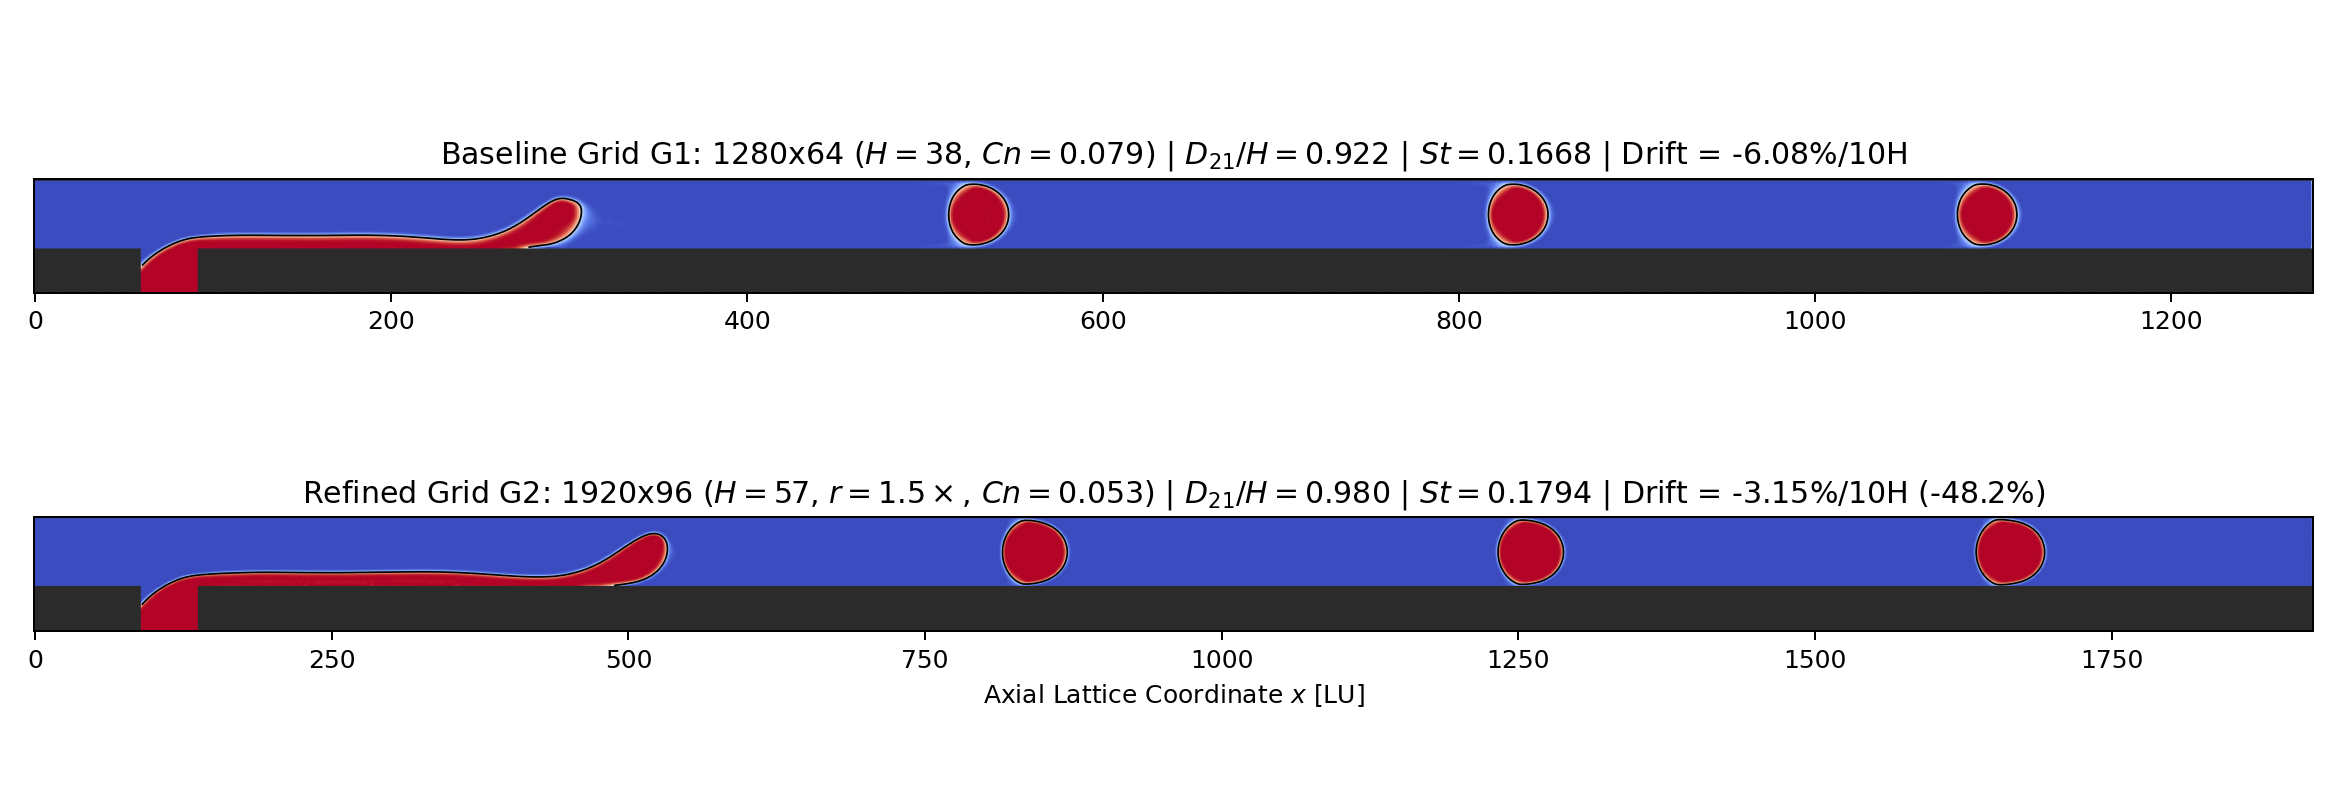
\includegraphics[width=\textwidth]{gis_fine/gis_comparison.png}
    \caption{Visual comparison of final phase-field topology at equivalent dimensionless time between baseline grid $G_1$ ($1280 \times 64$, $t = 36\,000$) and refined grid $G_2$ ($1920 \times 96$, $t = 66\,000$).}
    \label{fig:gis}
\end{figure}

\begin{table}[H]
\caption{Grid Independence Study metrics ($G_1$ vs. $G_2$, $r = 1.5$, MRT operator, $F_s = 3.0$ for two-grid GCI).}
\label{tab:gis}
\hspace{-1.5cm}
\begin{tabular}{@{}lccccc@{}}
\toprule
\textbf{Metric} & \textbf{$G_1$ ($1280 \times 64$)} & \textbf{$G_2$ ($1920 \times 96$)} & \textbf{Rel. Change} & \textbf{Richardson ($p=2$)} & \textbf{$\mathrm{GCI}_{\mathrm{fine}}$} \\
\midrule
$D_{21} / H$ [-] & $0.9220$ & $0.9802$ & $+5.94\%$ & $1.0268$ & $14.25\%$ \\
$L_b / H$ [-] & $6.3680$ & $6.8860$ & $+7.52\%$ & $7.3004$ & $18.05\%$ \\
Strouhal $St$ [-] & $0.1668$ & $0.1794$ & $+7.02\%$ & $0.1895$ & $16.86\%$ \\
Aspect Ratio $AR$ [-] & $1.0100$ & $1.0620$ & $+4.90\%$ & $1.1036$ & $11.75\%$ \\
\midrule
Mass Drift [\% / $10H$] & $-6.08\%$ & $-3.15\%$ & $-48.19\%$ & $p_{\mathrm{eff}} = 1.62$ & --- \\
Steady Drop Std [\%] & $2.55\%$ & $2.01\%$ & $-21.18\%$ & --- & --- \\
GPU Runtime (GTX 745) & $2.38\text{ min}$ & $\sim 9.8\text{ min}$ & $4.1\times$ cost & --- & --- \\
\bottomrule
\end{tabular}
\end{table}

Figure~\ref{fig:gis} confirms identical macro-scale flow topology across both meshes: three detached droplets occupy matching dimensionless axial coordinates ($x/H \approx 14.0, 21.9, 28.9$). Quantitatively (Table~\ref{tab:gis}), reducing the Cahn number by $1.5\times$ cuts in-flight diameter drift nearly in half ($-48.19\%$, superlinear effective convergence order $p = 1.62$) and reduces droplet scatter from $2.55\%$ to $2.01\%$. The $+5.94\%$ shift in $D_{21}/H$ reflects the sharp-interface convergence of diffuse-interface models as $Cn \to 0$. Consequently, grid $G_1$ provides a $4.1\times$ computational speedup suitable for multi-point parametric sweeps with a quantified $\sim 6\%$ discretization offset.

% ==============================================================================
\section{Collision Operator Comparison: MRT vs. Cumulant}
% ==============================================================================

To assess whether higher-order Galilean invariance and independent bulk-viscosity relaxation improve accuracy without incurring mesh-refinement cost, the full benchmark suite and the baseline T-junction ($G_1$, $U_c = 0.028$) were re-executed using the Cumulant collision operator (\texttt{d2q9\_csf\_viscstep\_cumulant}). To ensure a fair comparison, the boundary buffer viscosity \texttt{nubuffer} (default $0.01$ in TCLB) was explicitly matched to the fluid viscosity ($\nu_c = 0.025$ in the injector and Poiseuille tests; $1/6$ in the static Laplace test).

\begin{figure}[H]
    \centering
    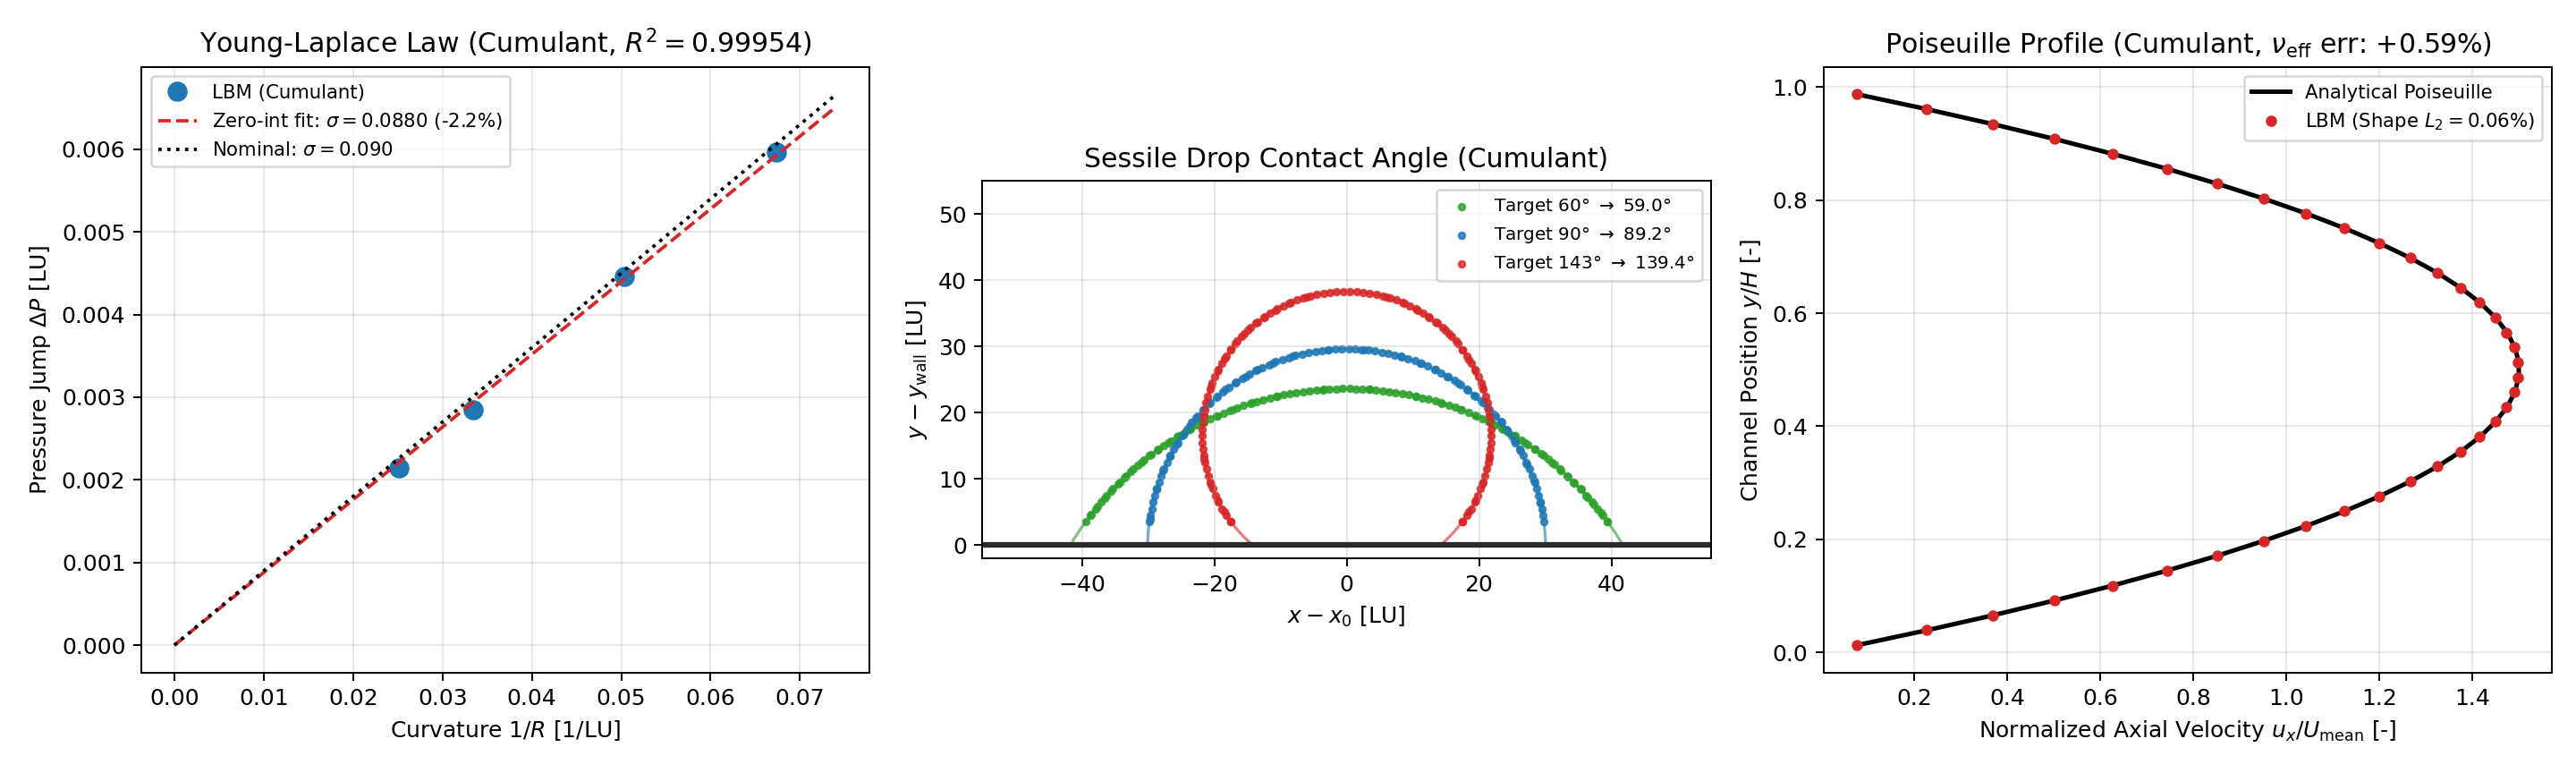
\includegraphics[width=\textwidth]{benchmarks_cumulant/validation_benchmarks.png}
    \caption{Component verification benchmarks executed with the Cumulant collision operator (\texttt{d2q9\_csf\_viscstep\_cumulant}).}
    \label{fig:bm_cum}
\end{figure}

\begin{figure}[H]
    \centering
    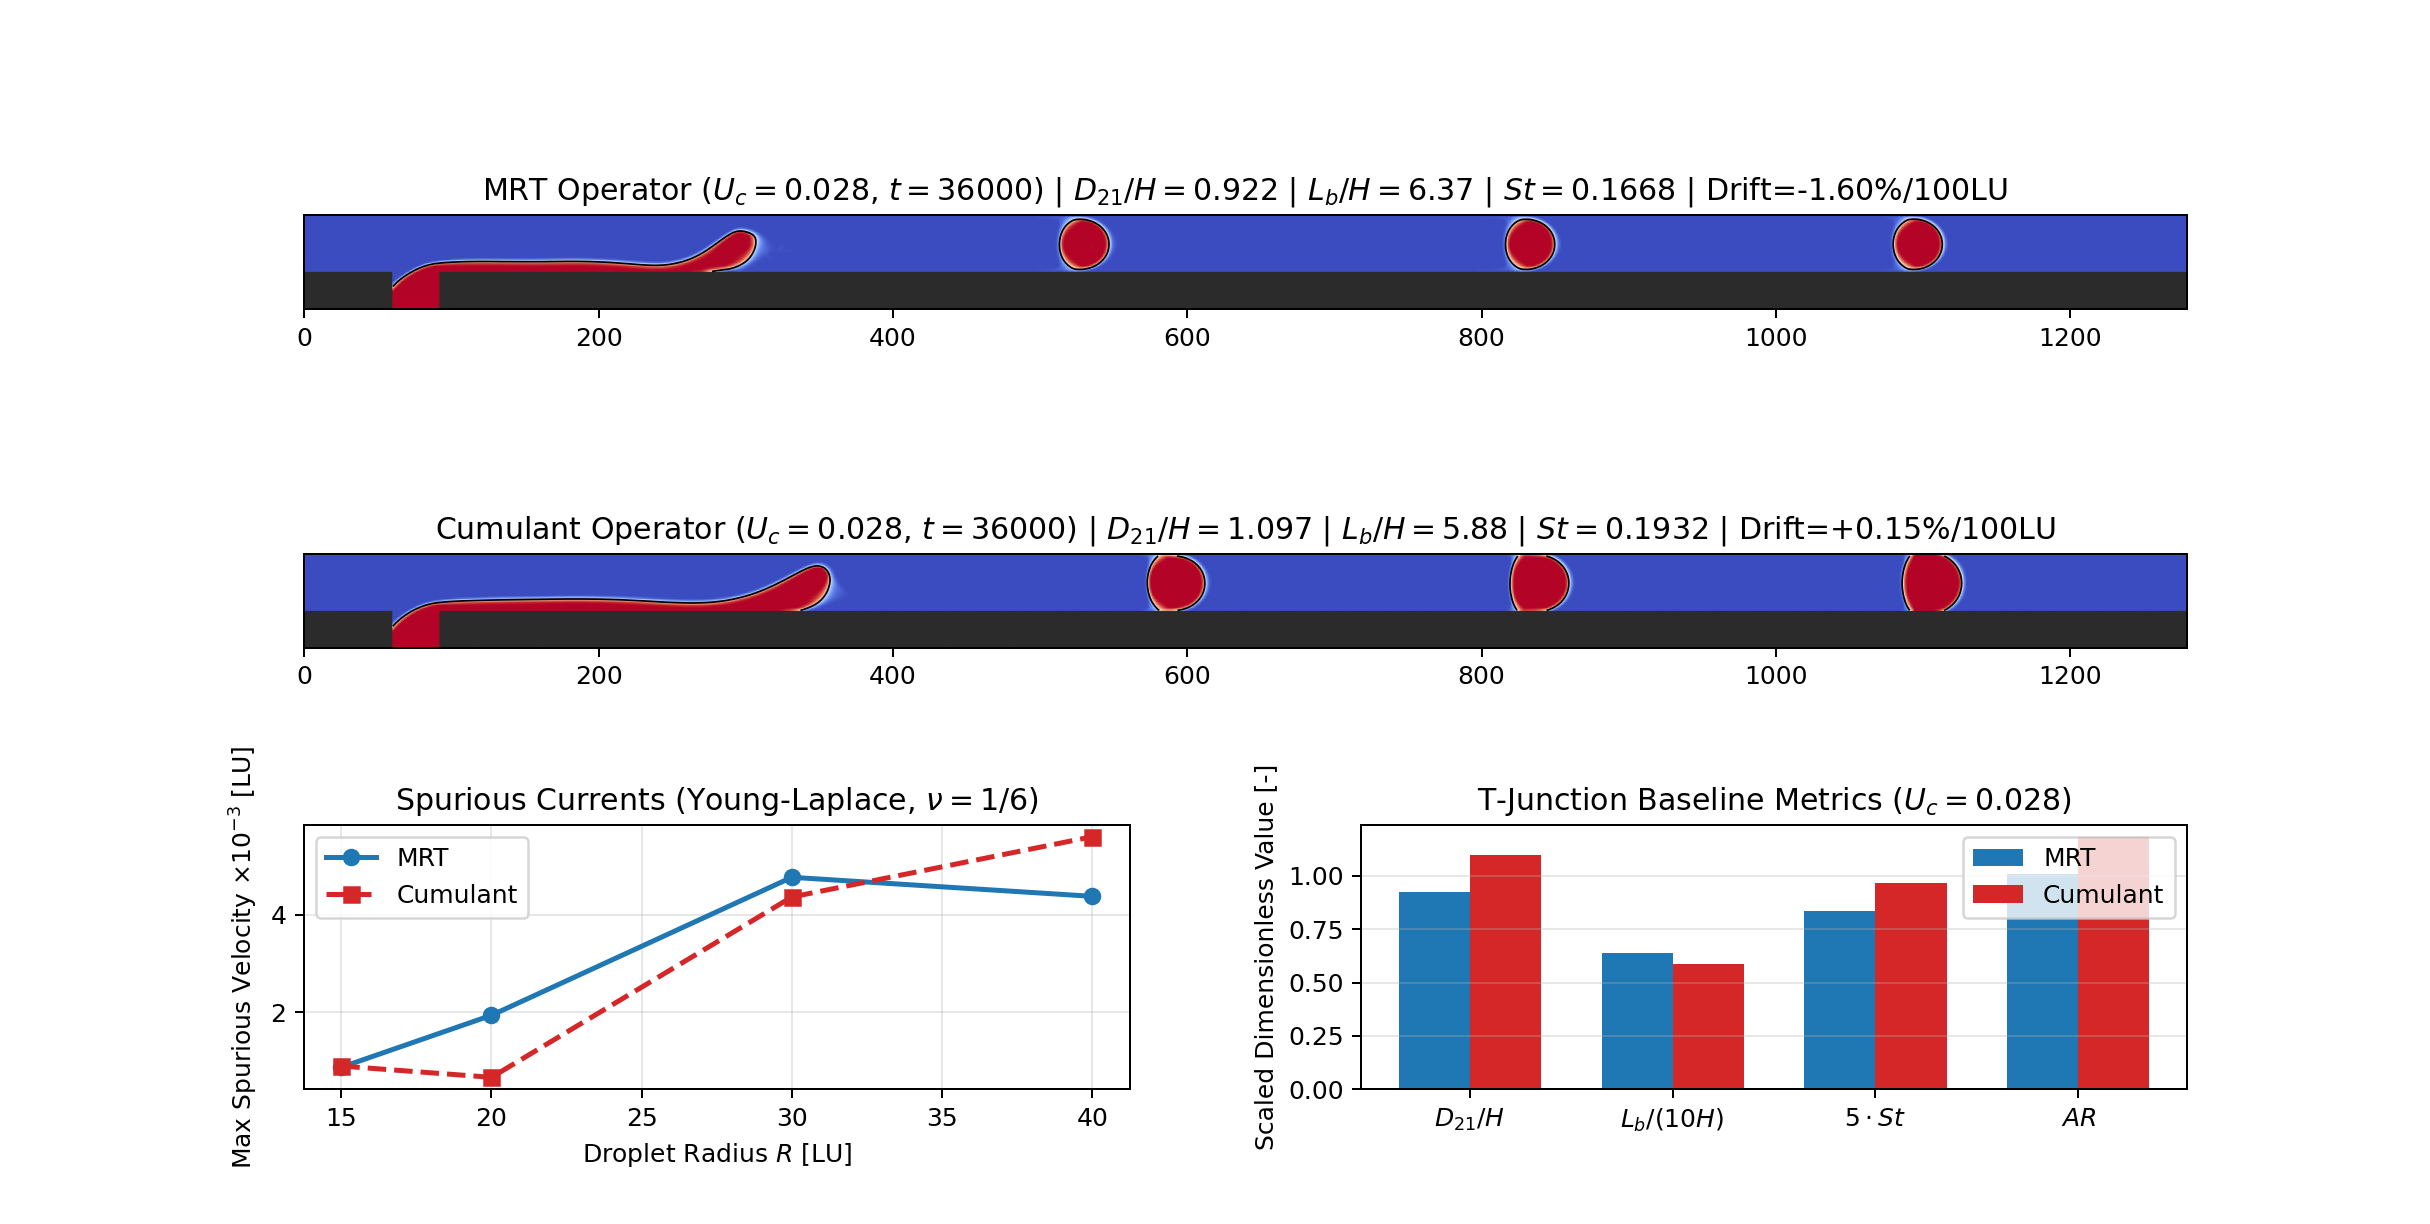
\includegraphics[width=\textwidth]{cumulant_cmp/mrt_vs_cumulant.png}
    \caption{Direct comparison between MRT and Cumulant collision operators: final phase-field snapshots at $t = 36\,000$ ($U_c = 0.028$), static Young-Laplace spurious currents vs. radius, and dimensionless baseline injector metrics.}
    \label{fig:mrt_vs_cum}
\end{figure}

\begin{table}[H]
\centering
\caption{Quantitative comparison between MRT and Cumulant collision operators on identical grids and parameters.}
\label{tab:mrt_vs_cum}
\small
\setlength{\tabcolsep}{5pt}
\begin{tabular}{@{}lccc@{}}
\toprule
\textbf{Metric} & \textbf{MRT} & \textbf{Cumulant} & \textbf{Difference} \\
\midrule
Young-Laplace $\sigma_{\mathrm{num}}$ ($\nu = 1/6$, zero-int) & $0.08857$ ($-1.59\%$) & $0.08798$ ($-2.25\%$) & $-0.67\%$ \\
Young-Laplace $\max|\mathbf{U}_{\mathrm{sp}}|$ ($\nu = 1/6$) & $0.00477\text{ LU}$ & $0.00560\text{ LU}$ & $+17.45\%$ \\
Low-$\nu$ Laplace $\sigma_{\mathrm{eff}}$ ($R=40$, $15\text{k}$ it) & $0.1035^*$ & $0.09226$ & $+2.51\%$ vs. $\sigma_{\mathrm{nom}}$ \\
Low-$\nu$ Laplace $\mathrm{std}(\rho_{\mathrm{in}})$ ($R=40$) & $1.4\text{--}17\times 10^{-4}$ & $2.1\times 10^{-5}$ & up to $80\times$ lower \\
Sessile drop ($\theta_{\mathrm{set}} = 143.24^\circ$) & $139.67^\circ$ & $139.44^\circ$ & $-0.23^\circ$ \\
Poiseuille shape $L_2$ / $\nu_{\mathrm{eff}}$ & $0.061\%$ / $0.02518$ & $0.060\%$ / $0.02515$ & Equivalent \\
\midrule
Injector $D_{21}/H$ ($U_c = 0.028$, $G_1$) & $0.9220$ & $1.0970$ & $+18.98\%$ \\
Injector $L_b/H$ & $6.3680$ & $5.8820$ & $-7.63\%$ \\
Injector Strouhal $St$ & $0.1668$ & $0.1932$ & $+15.83\%$ \\
Injector Aspect Ratio $AR$ & $1.010$ & $1.180$ & $+16.83\%$ \\
Injector Drop Scatter $D_{\mathrm{std}}$ & $2.55\%$ & $0.88\%$ & $-65.49\%$ \\
Injector Mass Drift [\% / $100\text{ LU}$] & $-1.60\%$ & $+0.15\%$ & $10.7\times$ lower \\
Droplet Mass Recovery $A_{\mathrm{drop}} / (Q_d T)$ & $46.3\%$ ($56.3\%$ on $G_2$) & $75.9\%$ (on $G_1$) & $+29.6\text{ pp}$ \\
\bottomrule
\end{tabular}

\vspace{4pt}
\begin{minipage}{0.96\textwidth}
\footnotesize $^*$MRT value at $t = 15\,500$ during persistent trapped acoustic oscillation ($30\text{k}$ time-averaged $\sigma = 0.0875 \pm 0.0263$).
\end{minipage}
\end{table}

Figures~\ref{fig:bm_cum}--\ref{fig:mrt_vs_cum} and Table~\ref{tab:mrt_vs_cum} reveal three decisive engineering findings:
\begin{enumerate}
    \item \textbf{Dramatic Mass Conservation Gain in Dynamic Flow:} Under identical grid resolution ($G_1$), switching from MRT to Cumulant reduces in-flight diameter drift by an order of magnitude ($-1.60\%$ to $+0.15\%/100\text{ LU}$), cuts droplet-to-droplet scatter by $65.5\%$ ($0.88\%$), and boosts volumetric mass recovery $A_{\mathrm{drop}} / (Q_d T)$ from $46.3\%$ to $75.9\%$. Notably, the Cumulant $D_{21}/H = 1.097$ on $G_1$ moves in the same direction as MRT mesh refinement ($0.922 \to 0.980 \to 1.027$ extrapolated), indicating that MRT on $G_1$ suffers from greater numerical mass dissipation during neck thinning and droplet transport.
    \item \textbf{Superior Acoustic Damping at Low Viscosity:} Because the Cumulant operator relaxes the trace of the stress tensor independently with $\omega_b = 1.0$ ($\nu_b = 1/6$) rather than coupling it to the low shear viscosity ($\nu_c = 0.025, \nu_d = 0.012$), radial acoustic modes in the low-viscosity Young-Laplace test ($R = 40$) decay cleanly to $\text{std}(\rho_{\mathrm{in}}) = 2.1 \times 10^{-5}$ with $\sigma_{\mathrm{eff}} = 0.09226$ ($+2.51\%$ error).
    \item \textbf{Limitation on Static Spurious Currents:} On the static $\nu = 1/6$ Young-Laplace benchmark, Cumulant does not suppress maximum spurious velocities ($0.0056\text{ LU}$ vs. $0.0048\text{ LU}$ for MRT). This confirms that static parasitic currents in \texttt{d2q9\_csf} are governed primarily by the discrete $2 \times 2$ curvature/force imbalance of the CSF stencil rather than velocity-space Galilean errors.
\end{enumerate}

% ==============================================================================
\section{Conclusions and Engineering Recommendations}
% ==============================================================================

A rigorous, GPU-accelerated LBM workflow for 2D T-junction micro-injector atomization was developed, verified, and quantitatively benchmarked in TCLB:
\begin{itemize}
    \item \textbf{Verified Solver Fidelity:} Component benchmarks confirm interfacial tension accuracy within $-1.59\%$ ($\sigma_{\mathrm{num}} = 0.08857$), effective viscosity within $+0.70\%$ ($\nu_{\mathrm{eff}} = 0.02518$), Poiseuille shape $L_2$ error of $0.061\%$, and an actual hydrophobic wall angle of $139.67^\circ$ (target $143.24^\circ$).
    \item \textbf{Validated Scaling Laws:} Across the steady dripping regime ($Ca \in [0.0064, 0.0117]$), droplet size and breakup length follow $D_{21}/H = 0.0149\,Ca^{-0.850}$ ($R^2 = 0.9997$) and $L_b/H = 0.0246\,Ca^{-1.140}$ ($R^2 = 0.9807$). At $Ca = 0.0050$ ($Q_d/Q_c = 0.37$), the injector transitions to confined Taylor slugging ($L_{\mathrm{slug}}/H = 1.263$) near the lower periodic stability limit.
    \item \textbf{Mesh and Operator Guidance:} While MRT on $1280 \times 64$ captures clean parametric trends at low GPU cost ($2.4\text{ min/case}$), the Cumulant operator is strongly recommended for production multiphase injector runs due to its $10.7\times$ reduction in mass drift, $65.5\%$ lower droplet scatter, and superior low-viscosity acoustic damping.
    \item \textbf{Future Extensions:} Extending the model to 3D (\texttt{d3q19\_csf} or \texttt{d3q27\_csf}) will introduce azimuthal neck curvature (accelerating pinch-off closer to the junction corner), while adopting a high-density-ratio formulation (\texttt{d2q9\_pf\_velocity} with an added \texttt{SVelocity} inlet and convective outflow) will enable realistic aerospace liquid-to-gas density contrasts ($\rho_d/\rho_c \sim 10^2\text{--}10^3$).
\end{itemize}

% ==============================================================================
\clearpage
\appendix
\section{Lattice Boltzmann Hydrodynamics: BGK, MRT, and Cumulant Operators}
\label{app:lbm}
% ==============================================================================

\subsection{Discrete Boltzmann Equation on the D2Q9 Lattice}

The Lattice Boltzmann Method (LBM) solves the mesoscopic evolution of particle distribution functions $f_i(\mathbf{x}, t)$ on a regular Cartesian lattice rather than discretizing the macroscopic Navier-Stokes equations directly. On the standard two-dimensional nine-velocity lattice (D2Q9), the discrete velocities $\mathbf{c}_i$ ($i = 0, \dots, 8$) and quadrature weights $w_i$ are:
\begin{equation}
    \mathbf{c}_i =
    \begin{cases}
        (0, 0), & i = 0, \quad w_0 = \frac{4}{9}, \\
        (\pm 1, 0), (0, \pm 1), & i = 1\dots 4, \quad w_i = \frac{1}{9}, \\
        (\pm 1, \pm 1), & i = 5\dots 8, \quad w_i = \frac{1}{36},
    \end{cases}
\end{equation}
with lattice speed of sound $c_s = 1/\sqrt{3}$ ($\Delta x = \Delta t = 1$). The evolve step splits into local collision and exact nearest-neighbor streaming:
\begin{equation}
    f_i(\mathbf{x} + \mathbf{c}_i, t + 1) = f_i(\mathbf{x}, t) + \Omega_i(\mathbf{f}) + S_i(\mathbf{F}),
\end{equation}
where $\Omega_i$ is the collision operator and $S_i(\mathbf{F})$ incorporates the external body force $\mathbf{F}$ (here, the CSF interfacial force). Macroscopic density $\rho$, pressure $P$, and fluid velocity $\mathbf{u}$ are recovered via low-order moments:
\begin{equation}
    \rho = \sum_{i=0}^{8} f_i, \qquad P = c_s^2 \rho = \frac{\rho}{3}, \qquad \mathbf{u} = \frac{1}{\rho}\left(\sum_{i=0}^{8} f_i \mathbf{c}_i + \frac{1}{2}\mathbf{F}\right).
\end{equation}

\subsection{BGK vs. Multi-Relaxation-Time (MRT) Collision}

The single-relaxation-time Bhatnagar-Gross-Krook (BGK) operator relaxes all populations toward the Maxwell-Boltzmann equilibrium $f_i^{\mathrm{eq}}$ at a single rate $\omega = (\tau)^{-1} = (3\nu + 1/2)^{-1}$. At low kinematic viscosities ($\nu \sim 0.01\text{--}0.025$, $\omega \to 2$), BGK suffers from severe checkerboard instabilities and amplified spurious currents near sharp interfaces.

To overcome these limitations, the TCLB \texttt{d2q9\_csf} model transforms distributions into orthogonal moment space via a transformation matrix $\mathbf{M}$ ($\mathbf{R} = \mathbf{M}\mathbf{f}$):
\begin{equation}
    \mathbf{R}^{\star} = \mathbf{R}^{\mathrm{eq}}(\rho, \mathbf{J} + \mathbf{F}) + \mathbf{S}\left(\mathbf{R} - \mathbf{R}^{\mathrm{eq}}(\rho, \mathbf{J})\right),
\end{equation}
where $\mathbf{J} = \sum_i f_i \mathbf{c}_i$ is the pre-collision momentum and $\mathbf{S} = \mathrm{diag}(s_k)$ is the relaxation matrix. Second-order stress moments relax with $s_2 = 1 - \omega$ (fixing kinematic viscosity $\nu = (1/\omega - 1/2)/3$), while third- and fourth-order non-hydrodynamic ghost moments relax aggressively ($s_3 = s_4 = 0$, i.e., full equilibrium reset in \texttt{d2q9\_csf}). Forcing is implemented via the Exact Difference Method (EDM), shifting equilibrium momentum from $\mathbf{J}$ to $\mathbf{J} + \mathbf{F}$ prior to transforming back ($\mathbf{f}^{\star} = \mathbf{M}^{-1}\mathbf{R}^{\star}$).

\textbf{Justification:} MRT was chosen as the baseline operator because aggressive damping of third- and fourth-order moments stabilizes sharp interfacial force gradients and viscosity contrasts ($\lambda = 0.48$) at low viscosity ($\omega_d = 1.866$) with minimal computational overhead on GPU.

\subsection{Cumulant Collision Operator}

In raw-moment MRT, higher-order moments depend nonlinearly on lower-order moments, introducing velocity-dependent ($O(u^3)$) violations of Galilean invariance and cross-talk between shear and bulk modes. The Cumulant LBM formulation transforms distributions into statistically independent central cumulants $c_{\alpha\beta}$ (logarithm of the central moment generating function) in the local moving reference frame of velocity $\mathbf{u}$:
\begin{equation}
    c_{20} + c_{02} \to (1 - \omega_b)(c_{20} + c_{02}) + \omega_b \frac{2}{3}, \qquad c_{20} - c_{02} \to (1 - \omega_s)(c_{20} - c_{02}), \qquad c_{11} \to (1 - \omega_s)c_{11},
\end{equation}
where $\omega_s = (3\nu + 1/2)^{-1}$ controls shear viscosity independently of the bulk relaxation rate $\omega_b = 1.0$ ($\nu_b = 1/6$). All third- and fourth-order cumulants ($c_{21}, c_{12}, c_{22}$) relax independently to zero at unit rate.

\textbf{Justification:} The Cumulant operator was selected for comparative evaluation specifically because (i) Galilean invariance in the moving frame minimizes advection-induced numerical diffusion of moving droplets, and (ii) independent bulk relaxation ($\omega_b = 1.0$) rapidly damps acoustic pressure waves at low shear viscosity without altering the physical Reynolds or Capillary numbers.

% ==============================================================================
\section{Conservative Phase-Field Model and CSF Interfacial Formulation}
\label{app:pf}
% ==============================================================================

\subsection{Conservative Allen-Cahn Interface Tracking}

The interface between the continuous phase ($\phi = -0.5$) and dispersed fuel ($\phi = +0.5$) is tracked by a second distribution function $h_i(\mathbf{x}, t)$ solving the conservative Allen-Cahn equation:
\begin{equation}
    \frac{\partial \phi}{\partial t} + \nabla \cdot (\phi \mathbf{u}) = \nabla \cdot \left[ M \left( \nabla \phi - 2W (1 - 4\phi^2)\,\hat{\mathbf{n}} \right) \right],
\end{equation}
where $\phi = \sum_i h_i$, $M$ is the mobility, $W$ is the inverse interface width parameter, and $\hat{\mathbf{n}} = \nabla \phi / |\nabla \phi|$ is the unit interface normal. In equilibrium across a flat interface, the diffusion flux balances the sharpening anti-diffusion flux, producing a hyperbolic-tangent profile:
\begin{equation}
    \phi(n) = -\frac{1}{2}\tanh\left(2 W (n - n_0)\right),
\end{equation}
whose $10\%\text{--}90\%$ transition thickness is $\xi_{90} = \operatorname{arctanh}(0.8)/W \approx 3.30\text{ LU}$ for $W = 0.333$. In the LBM scheme, $h_i$ undergoes BGK relaxation with $\omega_\phi = (3M + 1/2)^{-1}$ toward the modified equilibrium:
\begin{equation}
    h_i^{\mathrm{eq}} = \phi\,w_i \left[ 1 + 3(\mathbf{c}_i \cdot \mathbf{u}) + \frac{9}{2}(\mathbf{c}_i \cdot \mathbf{u})^2 - \frac{3}{2}|\mathbf{u}|^2 \right] + 3 M W (1 - 4\phi^2)\,w_i (\mathbf{c}_i \cdot \hat{\mathbf{n}}).
\end{equation}

\textbf{Justification:} Unlike Cahn-Hilliard models (which require fourth-order chemical potential derivatives and exhibit strong curvature-driven dissolution of small droplets), the conservative Allen-Cahn equation involves only second-order gradients, strictly conserves global $\sum \phi$ during collision and streaming, and allows independent control of interface thickness $W$ and mobility $M$.

\subsection{Continuum Surface Force (CSF) and Curvature Stencil}

Surface tension enters the momentum equation as a localized volumetric body force following Brackbill's CSF model:
\begin{equation}
    \mathbf{F}_{\mathrm{CSF}} = \sigma\,\kappa\,\nabla\phi, \qquad \kappa = -\nabla \cdot \left( \frac{\nabla\phi}{|\nabla\phi|} \right),
\end{equation}
active within the interfacial band $\phi^2 < 0.248$ (\texttt{SurfaceTensionDecay}). In \texttt{d2q9\_csf}, both $\nabla\phi$ and $\kappa$ are computed via bilinear polynomial reconstruction over the four $2 \times 2$ lattice boxes surrounding each fluid node, solved locally via Gram-Schmidt orthogonalization.

\subsection{Wetting Boundary Condition and Smooth Viscosity Interpolation}

At fluid nodes adjacent to solid walls, the geometric wall normal $\hat{\mathbf{n}}_w$ is precomputed and the polynomial system replaces wall-node values with the Neumann contact-angle constraint enforcing $\hat{\mathbf{n}} \cdot \hat{\mathbf{n}}_w = -\cos\theta$, where $\theta$ (\texttt{WettingAngle}) is measured inside the $\phi = +0.5$ fuel phase. Setting $\theta = 2.50\text{ rad}$ ($143.24^\circ$) renders the channel walls non-wetting to fuel, preventing wall pinning downstream of the nozzle. The near-wall force is scaled by \texttt{WallAdhesionDecay} $= 0.70$, which activates capillary detachment while preventing numerical blowup at sharp geometric corners.

To handle the viscosity contrast ($\nu_c = 0.025$, $\nu_d = 0.012$) stably even if $\phi$ slightly overshoots $[-0.5, +0.5]$, the \texttt{viscstep} compilation option interpolates the relaxation frequency via a bounded hyperbolic tangent:
\begin{equation}
    \omega(\phi) = \omega_c + (\omega_d - \omega_c)\,\frac{\tanh(\phi / \delta_\nu) - \tanh(-0.5 / \delta_\nu)}{\tanh(0.5 / \delta_\nu) - \tanh(-0.5 / \delta_\nu)}, \qquad \delta_\nu = 0.25.
\end{equation}

\textbf{Justification:} Standard linear viscosity interpolation in LBM becomes unbounded if local $\phi$ exceeds $\pm 0.5$ near pressure outlets or high-shear corners, causing $\omega \ge 2$ and immediate divergence. The bounded \texttt{viscstep} profile guarantees $\omega(\phi) \in [\min(\omega_c, \omega_d), \max(\omega_c, \omega_d)]$ everywhere in the domain.

% ==============================================================================
\section{Boundary Conditions, Dimensionless Groups, and Regime Theory}
\label{app:scaling}
% ==============================================================================

\subsection{Boundary Conditions}

Solid walls apply full halfway bounce-back ($f_{\bar{i}}(\mathbf{x}, t+1) = f_i^{\star}(\mathbf{x}, t)$, $h_{\bar{i}}(\mathbf{x}, t+1) = h_i^{\star}(\mathbf{x}, t)$), placing the effective zero-velocity wall midway between solid and fluid nodes ($y_{\mathrm{wall}} = y_{\mathrm{solid}} + 0.5$). Inlet velocities (\texttt{WVelocity}, \texttt{SVelocity}) and outlet pressure (\texttt{EPressure}) are enforced via Zou-He bounce-back of non-equilibrium populations, solving analytically for the three unknown incoming distributions at each boundary node.

\subsection{Governing Dimensionless Numbers}

Dynamic similarity between lattice units and physical aerospace micro-injectors is governed by the following dimensionless groups (with matched density $\rho_d / \rho_c = 1$ in \texttt{d2q9\_csf}):
\begin{align}
    Re_c &= \frac{U_c H}{\nu_c}, & Ca &= \frac{\rho \nu_c U_c}{\sigma}, & We &= \frac{\rho U_c^2 H}{\sigma} = Re_c\,Ca, \\
    St &= \frac{f H}{U_c} = \frac{H}{T_{P1} U_c}, & Pe &= \frac{U_c H}{M}, & Cn &= \frac{1}{W H}, & \lambda &= \frac{\nu_d}{\nu_c}.
\end{align}
Here $Ca$ measures viscous shear relative to capillary restoring forces, $We$ measures cross-flow inertia relative to surface tension, $St$ normalizes droplet shedding frequency, $Pe$ compares advection to phase-field diffusion, and $Cn$ quantifies the ratio of diffuse interface thickness to channel height.

\subsection{Constant-$\sigma$ Mesh Refinement Scaling}

In LBM grid independence studies, standard acoustic scaling ($\nu \propto r$, $\sigma \propto r$) increases $\sigma$ proportionally to the refinement ratio $r$, which can violate the capillary wave CFL condition $c_{\mathrm{cap}} = \sqrt{2\pi\sigma / \lambda_{\min}} < c_s$ or amplify near-wall forces. Diffusive scaling ($U \propto 1/r$, $\sigma \propto 1/r$) requires $r^2$ more iterations ($r^4$ total cost). In this work, constant-$\sigma$ scaling is applied for $r = 1.5$:
\begin{equation}
    H_2 = r H_1, \quad \sigma_2 = \sigma_1, \quad U_2 = \frac{U_1}{\sqrt{r}}, \quad \nu_2 = \nu_1\sqrt{r}, \quad M_2 = M_1\sqrt{r}, \quad N_{\mathrm{it},2} = r^{3/2} N_{\mathrm{it},1}.
\end{equation}
This scaling preserves $Re_c$, $Ca$, $We$, $Q_d/Q_c$, $Pe$, and $c_{\mathrm{cap}}$ identically across grids while reducing $Cn$ by $1/r$ at an intermediate computational cost ($r^{3.5} \approx 4.1\times$).

\subsection{Theoretical Droplet Formation Regimes}

In confined T-junctions, at very low capillary numbers ($Ca \lesssim 0.01$), the emerging dispersed finger blocks the main channel completely; breakup is then driven by upstream pressure buildup (\emph{squeezing}) rather than viscous shear, yielding a geometric scaling law independent of $Ca$:
\begin{equation}
    \frac{L_{\mathrm{slug}}}{H} = 1 + \alpha \frac{Q_d}{Q_c},
\end{equation}
where $\alpha \sim O(1)$ depends on the nozzle-to-channel aspect ratio $D/H$. As $Ca$ increases, viscous drag detaches the droplet before it can fully obstruct the channel (\emph{dripping}), and droplet diameter falls below $H$ following a power law $D/H \propto Ca^{-\beta}$. Note that in 2D simulations, the absence of out-of-plane azimuthal neck curvature ($1/R_\theta = 0$) delays pinch-off downstream compared to 3D channels and lowers the critical capillary number for jetting.

% ==============================================================================
\section{Verification Analytical Solutions and Uncertainty Metrics}
\label{app:vv}
% ==============================================================================

\subsection{Benchmark Analytical Solutions}

\begin{itemize}
    \item \textbf{2D Young-Laplace Law:} For a static 2D circular droplet of radius $R$ in mechanical equilibrium, the pressure jump across the interface equals $\Delta P = P_{\mathrm{in}} - P_{\mathrm{out}} = \sigma / R$. In LBM, $\Delta P = c_s^2 (\rho_{\mathrm{in}} - \rho_{\mathrm{out}}) = (\rho_{\mathrm{in}} - \rho_{\mathrm{out}})/3$.
    \item \textbf{Sessile Drop Geometry:} Neglecting gravity ($Bo = 0$), a droplet resting on a flat solid wall forms a circular cap of radius $R_{\mathrm{fit}}$ centered at $(x_0, y_0)$. The equilibrium contact angle measured inside the droplet is recovered from algebraic least-squares circle fitting to the sub-pixel $\phi = 0.0$ contour:
    \begin{equation}
        \theta_{\mathrm{num}} = \arccos\left( \frac{y_{\mathrm{wall}} - y_0}{R_{\mathrm{fit}}} \right), \qquad y_{\mathrm{wall}} = 0.5.
    \end{equation}
    \item \textbf{2D Planar Poiseuille Flow:} For steady laminar flow of mean velocity $U_{\mathrm{mean}}$ between stationary plates separated by $H$, the analytical velocity profile and axial density gradient are:
    \begin{equation}
        u_x(\eta) = 6 U_{\mathrm{mean}} \eta (1 - \eta), \quad \eta = \frac{y - 0.5}{H} \in (0, 1), \qquad \frac{\partial \rho}{\partial x} = -\frac{36 \nu U_{\mathrm{mean}}}{H^2}.
    \end{equation}
    Discrepancies are quantified using the discrete relative $L_2$ norm, $E_{L2} = \|\mathbf{u}_{\mathrm{sim}} - \mathbf{u}_{\mathrm{ana}}\|_2 / \|\mathbf{u}_{\mathrm{ana}}\|_2$.
\end{itemize}

\subsection{Droplet Sizing and Grid Convergence Index (GCI)}

Individual droplet sizes are reported via the 2D Sauter mean diameter $D_{21}$ (analogous to 3D $D_{32}$, representing the volume-to-surface-area ratio critical to spray evaporation):
\begin{equation}
    D_{21} = \frac{\sum_{k=1}^{N} D_{\mathrm{eq},k}^2}{\sum_{k=1}^{N} D_{\mathrm{eq},k}}, \qquad D_{\mathrm{eq},k} = 2\sqrt{\frac{A_k}{\pi}}.
\end{equation}
Using the standard Grid Convergence Index (GCI) formulation, for two grids ($G_1, G_2$) with refinement ratio $r = h_1/h_2 = 1.5$ and formal second-order LBM accuracy ($p = 2$), the Richardson-extrapolated continuum estimate $\phi_{\mathrm{ext}}$ and conservative fine-grid uncertainty $\mathrm{GCI}_{\mathrm{fine}}$ (using safety factor $F_s = 3.0$ for two-grid studies) are defined as:
\begin{equation}
    \phi_{\mathrm{ext}} = \phi_2 + \frac{\phi_2 - \phi_1}{r^p - 1}, \qquad \mathrm{GCI}_{\mathrm{fine}} = \frac{F_s}{r^p - 1} \left| \frac{\phi_2 - \phi_1}{\phi_2} \right| \times 100\%.
\end{equation}
For error quantities that converge toward zero (such as in-flight mass drift $e$), the observed convergence order is evaluated directly from $p_{\mathrm{eff}} = \ln(|e_1|/|e_2|) / \ln(r)$.

\begin{comment}

\end{comment}

\end{document}